%-*-latex-*-
\sectionthree{Binary Search Tree}
\begin{python0}
from solutions import *; clear()
\end{python0}

A \defone{binary search tree} (BST)
is a binary tree where every node contains data in such a way that
\begin{itemize}
\li $T$ is an empty tree, or
\li The values in the nodes of $T$ are distinct
    and if $x$ is the data in the root of $T$, then every
    value in the left subtree of $x$ is less than $x$
    and every value in the right subtree of $x$ is greater than $x$.
    Furthermore, every node in $T$ satisfies the above
    property.
\end{itemize}

Here's a BST:

\begin{center}

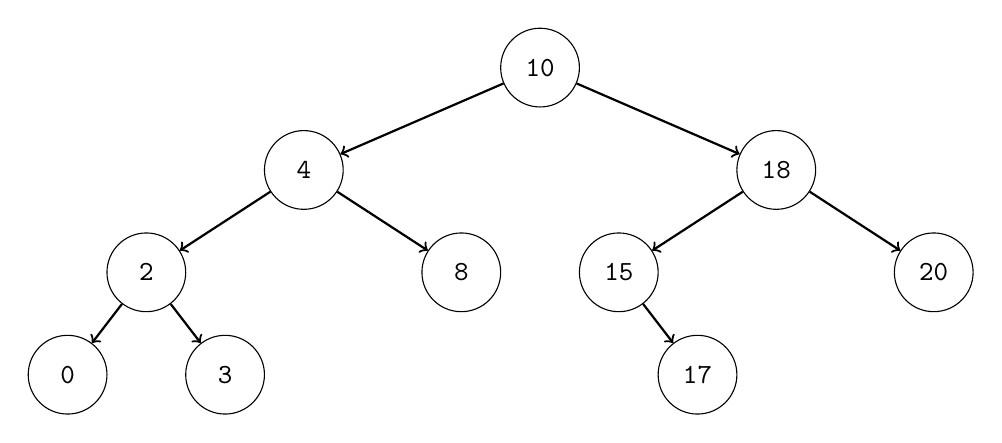
\begin{tikzpicture}
\node at (6,-1.3) [circle,draw,minimum size=10mm] (a) {\texttt{10}};
\node at (3,-2.6) [circle,draw,minimum size=10mm] (b) {\texttt{4}};
\node at (9,-2.6) [circle,draw,minimum size=10mm] (d) {\texttt{18}};
\node at (1,-3.9000000000000004) [circle,draw,minimum size=10mm] (e) {\texttt{2}};
\node at (5,-3.9000000000000004) [circle,draw,minimum size=10mm] (f) {\texttt{8}};
\node at (7,-3.9000000000000004) [circle,draw,minimum size=10mm] (h) {\texttt{15}};
\node at (11,-3.9000000000000004) [circle,draw,minimum size=10mm] (j) {\texttt{20}};
\node at (0,-5.2) [circle,draw,minimum size=10mm] (k) {\texttt{0}};
\node at (2,-5.2) [circle,draw,minimum size=10mm] (l) {\texttt{3}};
\node at (8,-5.2) [circle,draw,minimum size=10mm] (m) {\texttt{17}};
\draw [->,thick] (a) -- (b);
\draw [->,thick] (a) -- (d);
\draw [->,thick] (b) -- (e);
\draw [->,thick] (b) -- (f);
\draw [->,thick] (d) -- (h);
\draw [->,thick] (d) -- (j);
\draw [->,thick] (e) -- (k);
\draw [->,thick] (e) -- (l);
\draw [->,thick] (h) -- (m);

;
\end{tikzpicture}
    
\end{center}



Of course if you perform an infix traversal of a BST and print the
nodes that you visit during the traversal, you will get an ascending
sequence of values taken from tree.


\begin{ex}
How many ways are there to build a BST given
\begin{tightlist}
  \li 2 key values?
  \li 3 key values?
  \li 4 key values?
\end{tightlist}
\qed
\end{ex}
  
\newpage
\subsection{Search}

The point of the BST is to aid in search.
For instance if you're search for \verb!17!, 
you start at the root and see the value \verb!10!.
Since the tree is a BST and you're looking for \verb!17!,
then if it's in the tree, it must be in the right subtree at \verb!10!.
Following the right subtree, we arrive at teh node with value \verb!18!.
Since 17 is less than 18, we follow the left subtree and arrive at 
\verb!15!.
Then following the right subtree, we arrive at \verb!17!.

Of course in this case the number of steps needed is the height of three.

Recall that if $n$ is the number of nodes in a BST
and suppose the height is $h$.
From
\[
h + 1 \leq n \leq 2^{h+1} - 1
\]
we see that 
if the tree has roughly the same number of nodes on the right 
as on the left for each node, i.e., when the tree is balanced. 
the search 
takes
\[
n = 2^{h + 1}
\]
i..e, 
\[
h + 1 = \lg n
\]
In the worst case search when
we see that the number of steps to search for a value is
\[
h + 1 = n 
\]
steps for instance when the BST looks like this

from latextool_basic import *
print(automata(layout="""
   D  E  F
""",
edges="D,$a$,D|D,$b$,E|E,$b$,F|F,$a$,D",
D='initial|accept|label=$q_3$',
E='label=$q_4$',
F='label=$q_5$',
))


This is the worst case, i.e., the worst runtime for BST search is
\[
O(n)
\]
The point is that if the tree is heavily \lq\lq unbalanced'',
i.e., all the nodes are always \lq\lq on the left'' or \lq\lq on the right''.
In the average case,
the BST is \lq\lq roughly'' balanced and therefore
the average runtime for BST search is
\[
O(\log n)
\]


\newpage
\begin{ex}
  
  Given this BST
  
\begin{center}
\begin{tikzpicture}[>=triangle 60,shorten >=0.5pt,node distance=2cm,auto,initial text=, double distance=2pt]
\node[state] (A) at (  0,  0) {$a$};
\node[state] (B) at (  3,  0) {$b$};
\node[state] (F) at (  6,  0) {$f$};
\node[state] (C) at (  0, -2) {$c$};
\node[state] (D) at (  3, -2) {$d$};
\node[state] (E) at (  6, -2) {$e$};

\path[->]
(A) edge [loop above] node {} ()
(A) edge [bend left=0,pos=0.5,above] node {} (B)
(B) edge [bend left=0,pos=0.5] node {} (D)
(B) edge [bend left=0,pos=0.5,above] node {} (E)
(C) edge [bend left=0,pos=0.5,above] node {} (B)
(C) edge [bend left=0,pos=0.5,above] node {} (D)
(D) edge [bend left=0,pos=0.5,above] node {} (E)

;
\end{tikzpicture}
\end{center}
    

what nodes were visited while performing a BST search for
the following cases: 4, 9, 20?
\qed
\end{ex}


\newpage
Here's the algorithm to perform a search in a BST:
\begin{console}
ALGORITHM: BST-SEARCH
INPUT: node
       key (the target)

if node is NONE:
    return NOT FOUND

if node.key is key:
    return node
else:
    if key < node.key:
        BST-SEARCH(node.left, key)
    else data > node.data:
        BST-SEARCH(node.right, key)
\end{console}

Here's a version that's close to C++:
\begin{console}
Node * bst_search(Node * p, int key)
{
    if p is NULL, return NULL

    if p->key is key
        return p
    else if key < p->key
        bst_search(p->left, key)
    else key > p->key
        bst_search(p->right, key)
}
\end{console}


\newpage
\begin{ex}
Implement the following
C++ function so that it performs a BST search
and returns the pointer to the node with the
given key value; \verb!NULL! is returned is the
key value is not found in the BST.
\begin{Verbatim}[frame=single]
Node * bst_search(Node * p, int key);
\end{Verbatim}
\end{ex}




\newpage
\subsection{Insert}

Of course when you insert a value into a BST, 
you have to make sure it's still a BST so that search for it
later is still fast.
Note that a BST is a self-organizing container.

\begin{console}
ALGORITHM: BST-INSERT
INPUT: node
       newvalue

if node is NONE:
    set node to a new node with key newvalue
    return
 
if node.key < newvalue:
    if node.right is NONE:
        create a new node with key newvalue and
        make it the left child of node
    else:
        BST-INSERT(node.right, newvalue)
else if node.key > newvalue:
    if node.left is NONE:
        create a new node with key newvalue and
        make it the right child of node
    else:
        BST-INSERT(node.left, newvalue)
else:
    return ERROR -- DUPLICATE NODE
\end{console}

The runtime behavior is similar to the runtime behavior for
BST search.
The worst case is
\[
O(n)
\]
The average runtime is
\[
O(\log n)
\]

In the above, I'm assuming that the key values in the BST
are unique.

\newpage
\begin{ex}
Now C++ pseudocode this time ... implement the following C++ functions
\begin{Verbatim}[frame=single]
void bst_insert(Node ** p, int key);
void bst_insert(Node *& p, int key);
\end{Verbatim}
(Just for practice, throw an exception when there's a duplicate key.)
\qed
\end{ex}


\newpage
\begin{ex}
The above algorithms are rather similar.
Can you find a useful helper function?
(Instead of a pointer \verb!q! walking down the tree, you need another
pointer \verb!r! that is \lq\lq behind'' \verb!q!.)
\qed
\end{ex}

\newpage
\subsection{Delete}

But what about node deletion?
No problem when deleting leaves of course.
What about deleting a non-leaf node?
Look at this again:

\begin{center}
\begin{tikzpicture}
\draw[line width=0.03cm,red,<->] (5) to [bend left=60]  (7);

\fill[blue!10] (0.0, 0.0) circle (0.35);
\node [line width=0.03cm,black,minimum size=0.6699999999999999cm,draw,circle] at (0.0,0.0)(20){};\draw (0.0, 0.0) node[color=black] {\texttt{20}};
\fill[blue!10] (-1.9, -1.0) circle (0.35);
\node [line width=0.03cm,black,minimum size=0.6699999999999999cm,draw,circle] at (-1.9,-1.0)(10){};\draw (-1.9, -1.0) node[color=black] {\texttt{10}};
\fill[blue!10] (1.9, -1.0) circle (0.35);
\node [line width=0.03cm,black,minimum size=0.6699999999999999cm,draw,circle] at (1.9,-1.0)(5){};\draw (1.9, -1.0) node[color=black] {\texttt{5}};
\fill[blue!10] (-2.85, -2.0) circle (0.35);
\node [line width=0.03cm,black,minimum size=0.6699999999999999cm,draw,circle] at (-2.85,-2.0)(9){};\draw (-2.85, -2.0) node[color=black] {\texttt{9}};
\fill[blue!10] (-0.95, -2.0) circle (0.35);
\node [line width=0.03cm,black,minimum size=0.6699999999999999cm,draw,circle] at (-0.95,-2.0)(1){};\draw (-0.95, -2.0) node[color=black] {\texttt{1}};
\fill[blue!10] (0.95, -2.0) circle (0.35);
\node [line width=0.03cm,black,minimum size=0.6699999999999999cm,draw,circle] at (0.95,-2.0)(0){};\draw (0.95, -2.0) node[color=black] {\texttt{0}};
\fill[blue!10] (2.85, -2.0) circle (0.35);
\node [line width=0.03cm,black,minimum size=0.6699999999999999cm,draw,circle] at (2.85,-2.0)(7){};\draw (2.85, -2.0) node[color=black] {\texttt{7}};
\fill[blue!10] (-3.33, -3.0) circle (0.35);
\node [line width=0.03cm,black,minimum size=0.6699999999999999cm,draw,circle] at (-3.33,-3.0)(2){};\draw (-3.33, -3.0) node[color=black] {\texttt{2}};\draw[line width=0.03cm,black] (20) to  (10);
\draw[line width=0.03cm,black] (20) to  (5);
\draw[line width=0.03cm,black] (10) to  (9);
\draw[line width=0.03cm,black] (10) to  (1);
\draw[line width=0.03cm,black] (5) to  (0);
\draw[line width=0.03cm,black] (5) to  (7);
\draw[line width=0.03cm,black] (9) to  (2);
\end{tikzpicture}

\end{center}



If I delete \verb!4!, maybe we can move \verb!8! up to occupy
the position taken up by \verb!4!:
\begin{center}
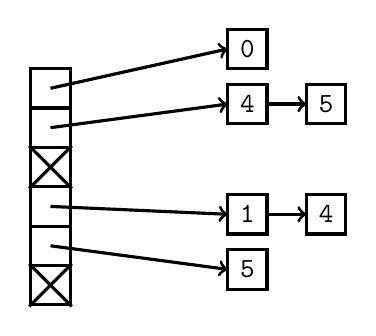
\begin{tikzpicture}

\draw (0.25, -0.25)
  node[draw, line width=0.04cm, , color=black,
       rounded corners=0cm, inner sep=0cm] {

\begin{minipage}[t][0.5cm]{0.5cm}
\mbox{}

\end{minipage}

};
\draw (0.25, -0.75)
  node[draw, line width=0.04cm, , color=black,
       rounded corners=0cm, inner sep=0cm] {

\begin{minipage}[t][0.5cm]{0.5cm}
\mbox{}

\end{minipage}

};
\draw (0.25, -1.25)
  node[draw, line width=0.04cm, , color=black,
       rounded corners=0cm, inner sep=0cm] {

\begin{minipage}[t][0.5cm]{0.5cm}
\mbox{}

\end{minipage}

};
\draw (0.25, -1.75)
  node[draw, line width=0.04cm, , color=black,
       rounded corners=0cm, inner sep=0cm] {

\begin{minipage}[t][0.5cm]{0.5cm}
\mbox{}

\end{minipage}

};
\draw (0.25, -2.25)
  node[draw, line width=0.04cm, , color=black,
       rounded corners=0cm, inner sep=0cm] {

\begin{minipage}[t][0.5cm]{0.5cm}
\mbox{}

\end{minipage}

};
\draw (0.25, -2.75)
  node[draw, line width=0.04cm, , color=black,
       rounded corners=0cm, inner sep=0cm] {

\begin{minipage}[t][0.5cm]{0.5cm}
\mbox{}

\end{minipage}

};\draw[line width=0.04cm,black] (-0.02,-0.98) to  (0.52,-1.52);
\draw[line width=0.04cm,black] (0.52,-0.98) to  (-0.02,-1.52);
\draw[line width=0.04cm,black] (-0.02,-2.48) to  (0.52,-3.02);
\draw[line width=0.04cm,black] (0.52,-2.48) to  (-0.02,-3.02);

\draw (2.75, 0.24999999999999992)
  node[draw, line width=0.04cm, , color=black,
       rounded corners=0cm, inner sep=0cm] {

\begin{minipage}[t][0.5cm]{0.5cm}
\mbox{}

\end{minipage}

};\draw (2.75, 0.24999999999999992) node[color=black] {{\texttt{0}}};
\draw (2.75, -0.45000000000000007)
  node[draw, line width=0.04cm, , color=black,
       rounded corners=0cm, inner sep=0cm] {

\begin{minipage}[t][0.5cm]{0.5cm}
\mbox{}

\end{minipage}

};\draw (2.75, -0.45000000000000007) node[color=black] {{\texttt{4}}};
\draw (3.75, -0.45000000000000007)
  node[draw, line width=0.04cm, , color=black,
       rounded corners=0cm, inner sep=0cm] {

\begin{minipage}[t][0.5cm]{0.5cm}
\mbox{}

\end{minipage}

};\draw (3.75, -0.45000000000000007) node[color=black] {{\texttt{5}}};
\draw (2.75, -1.85)
  node[draw, line width=0.04cm, , color=black,
       rounded corners=0cm, inner sep=0cm] {

\begin{minipage}[t][0.5cm]{0.5cm}
\mbox{}

\end{minipage}

};\draw (2.75, -1.85) node[color=black] {{\texttt{1}}};
\draw (3.75, -1.85)
  node[draw, line width=0.04cm, , color=black,
       rounded corners=0cm, inner sep=0cm] {

\begin{minipage}[t][0.5cm]{0.5cm}
\mbox{}

\end{minipage}

};\draw (3.75, -1.85) node[color=black] {{\texttt{4}}};
\draw (2.75, -2.55)
  node[draw, line width=0.04cm, , color=black,
       rounded corners=0cm, inner sep=0cm] {

\begin{minipage}[t][0.5cm]{0.5cm}
\mbox{}

\end{minipage}

};\draw (2.75, -2.55) node[color=black] {{\texttt{5}}};\draw[line width=0.04cm,black,->] (0.25,-0.25) to  (2.5,0.25);
\draw[line width=0.04cm,black,->] (0.25,-0.75) to  (2.5,-0.45);
\draw[line width=0.04cm,black,->] (3.0,-0.45) to  (3.5,-0.45);
\draw[line width=0.04cm,black,->] (0.25,-1.75) to  (2.5,-1.85);
\draw[line width=0.04cm,black,->] (3.0,-1.85) to  (3.5,-1.85);
\draw[line width=0.04cm,black,->] (0.25,-2.25) to  (2.5,-2.55);
\end{tikzpicture}

\end{center}


Why is that possible?
Because \verb!8! has no left child.
If \verb!8! has a left child, when you move \verb!8! up,
its left child will \lq\lq collide'' with \verb!2!.
Right?
Think about this:
if \verb!8! has a right child (or even a right subtree) but no 
left child,
you can \textit{still} move \verb!8! up to \verb!4!'s place.

But what if I want to move something up from the left of \verb!4!?
For instance, remember that we do want our BSTs to be
as balanced as possible. 
Since there are more node on the left of \verb!4!,
maybe we want to move something on the left of \verb!4! up
to \verb!4!'s position instead of using some node on the 
right. How are we going to do that???

Furthermore, what if I need to delete \verb!10!?
You see that it's not so clear what we should do ...

You can of course do an inorder traversal of the tree
to create an array/vector/list of the nodes, omitting \verb!10!,
and then rebuild the tree.
But that's extremely costly!!!
We want to disrupt the tree minimally!!!

If you think about it, you see that
to delete root \verb!10!,
you want to you can move the \verb!8! to the 
same place as the root
or move \texttt{15} to the root's place.
Why?
Two reasons:
because they have at most
one child and because they are values closest to 
\verb!10!!!!
The fact that they have at most one child
means that their single child can move to their place without
worry about collisions when they are moved to their new places.
For instance, see \texttt{17} the right child of \texttt{15} above.
The fact that they are values closest to \verb!10! means that
there won't be nodes between them and \verb!10! that might be
disrupted because of the move.
Right?

In the case of moving \verb!8!, we get this
from latextool_basic import *
print(automata(layout="""
   D  E  F

      C1 D1
   A1 
      G1
""",
edges="D,$a$,D|D,$b$,E|E,$b$,F|F,$a$,D|A1,$b$,C1|C1,$a$,D1|D1,$b$,A1|A1,$a$,G1|G1,$b$,A1|D,$\ep$,A1",
D='initial|label=$q_3$',
E='label=$q_4$',
F='label=$q_5$',
A1='accept|label=$q_7$',
C1='label=$q_9$',
D1='label=$q_{10}$',
G1='label=$q_{13}$',
))


and in the case of moving \texttt{15}, we get this:
\begin{center}
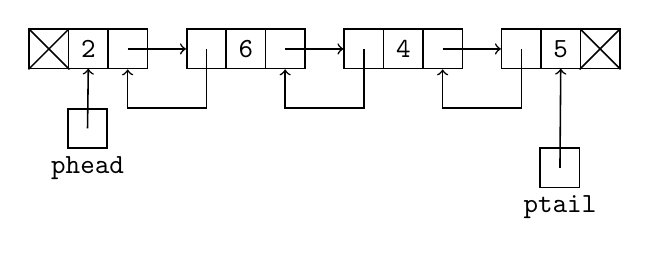
\begin{tikzpicture}

\draw (0.25, 0.25)
  node[draw, line width=0.02cm, , color=black,
       rounded corners=0cm, inner sep=0cm] {

\begin{minipage}[t][0.5cm]{0.5cm}
\mbox{}

\end{minipage}

};\draw (0.25, 0.25) node[color=black] {{\texttt{}}};
\draw (0.75, 0.25)
  node[draw, line width=0.02cm, , color=black,
       rounded corners=0cm, inner sep=0cm] {

\begin{minipage}[t][0.5cm]{0.5cm}
\mbox{}

\end{minipage}

};\draw (0.75, 0.25) node[color=black] {{\texttt{2}}};
\draw (1.25, 0.25)
  node[draw, line width=0.02cm, , color=black,
       rounded corners=0cm, inner sep=0cm] {

\begin{minipage}[t][0.5cm]{0.5cm}
\mbox{}

\end{minipage}

};\draw (1.25, 0.25) node[color=black] {{\texttt{}}};
\draw (2.25, 0.25)
  node[draw, line width=0.02cm, , color=black,
       rounded corners=0cm, inner sep=0cm] {

\begin{minipage}[t][0.5cm]{0.5cm}
\mbox{}

\end{minipage}

};\draw (2.25, 0.25) node[color=black] {{\texttt{}}};
\draw (2.75, 0.25)
  node[draw, line width=0.02cm, , color=black,
       rounded corners=0cm, inner sep=0cm] {

\begin{minipage}[t][0.5cm]{0.5cm}
\mbox{}

\end{minipage}

};\draw (2.75, 0.25) node[color=black] {{\texttt{6}}};
\draw (3.25, 0.25)
  node[draw, line width=0.02cm, , color=black,
       rounded corners=0cm, inner sep=0cm] {

\begin{minipage}[t][0.5cm]{0.5cm}
\mbox{}

\end{minipage}

};\draw (3.25, 0.25) node[color=black] {{\texttt{}}};
\draw (4.25, 0.25)
  node[draw, line width=0.02cm, , color=black,
       rounded corners=0cm, inner sep=0cm] {

\begin{minipage}[t][0.5cm]{0.5cm}
\mbox{}

\end{minipage}

};\draw (4.25, 0.25) node[color=black] {{\texttt{}}};
\draw (4.75, 0.25)
  node[draw, line width=0.02cm, , color=black,
       rounded corners=0cm, inner sep=0cm] {

\begin{minipage}[t][0.5cm]{0.5cm}
\mbox{}

\end{minipage}

};\draw (4.75, 0.25) node[color=black] {{\texttt{4}}};
\draw (5.25, 0.25)
  node[draw, line width=0.02cm, , color=black,
       rounded corners=0cm, inner sep=0cm] {

\begin{minipage}[t][0.5cm]{0.5cm}
\mbox{}

\end{minipage}

};\draw (5.25, 0.25) node[color=black] {{\texttt{}}};
\draw (6.25, 0.25)
  node[draw, line width=0.02cm, , color=black,
       rounded corners=0cm, inner sep=0cm] {

\begin{minipage}[t][0.5cm]{0.5cm}
\mbox{}

\end{minipage}

};\draw (6.25, 0.25) node[color=black] {{\texttt{}}};
\draw (6.75, 0.25)
  node[draw, line width=0.02cm, , color=black,
       rounded corners=0cm, inner sep=0cm] {

\begin{minipage}[t][0.5cm]{0.5cm}
\mbox{}

\end{minipage}

};\draw (6.75, 0.25) node[color=black] {{\texttt{5}}};
\draw (7.25, 0.25)
  node[draw, line width=0.02cm, , color=black,
       rounded corners=0cm, inner sep=0cm] {

\begin{minipage}[t][0.5cm]{0.5cm}
\mbox{}

\end{minipage}

};\draw (7.25, 0.25) node[color=black] {{\texttt{}}};\draw[line width=0.02cm,black,->] (1.25,0.25) to  (1.99,0.25);
\draw[line width=0.02cm,black,->] (3.25,0.25) to  (3.99,0.25);
\draw[line width=0.02cm,black,->] (2.25,0.25) to  (2.25,-0.5) to  (1.25,-0.5) to  (1.25,-0.01);
\draw[line width=0.02cm,black,->] (5.25,0.25) to  (5.99,0.25);
\draw[line width=0.02cm,black,->] (4.25,0.25) to  (4.25,-0.5) to  (3.25,-0.5) to  (3.25,-0.01);
\draw[line width=0.02cm,black,->] (6.25,0.25) to  (6.25,-0.5) to  (5.25,-0.5) to  (5.25,-0.01);
\draw[line width=0.02cm,black] (-0.01,0.51) to  (0.51,-0.01);
\draw[line width=0.02cm,black] (0.51,0.51) to  (-0.01,-0.01);
\draw[line width=0.02cm,black] (6.99,0.51) to  (7.51,-0.01);
\draw[line width=0.02cm,black] (7.51,0.51) to  (6.99,-0.01);

\draw (0.74, -0.76)
  node[draw, line width=0.02cm, , color=black,
       rounded corners=0cm, inner sep=0cm] {

\begin{minipage}[t][0.5cm]{0.5cm}
\mbox{}

\end{minipage}

};\draw (0.74, -0.76) node[color=black] {{\texttt{}}};
\draw (0.74, -1.26)
  node[draw, line width=0.02cm, , color=white,
       rounded corners=0cm, inner sep=0cm] {

\begin{minipage}[t][0.1cm]{0.1cm}
\mbox{}

\end{minipage}

};\draw (0.74, -1.26) node[color=black] {{\texttt{phead}}};\draw[line width=0.02cm,black,->] (0.74,-0.76) to  (0.75,0);

\draw (6.74, -1.26)
  node[draw, line width=0.02cm, , color=black,
       rounded corners=0cm, inner sep=0cm] {

\begin{minipage}[t][0.5cm]{0.5cm}
\mbox{}

\end{minipage}

};\draw (6.74, -1.26) node[color=black] {{\texttt{}}};
\draw (6.74, -1.76)
  node[draw, line width=0.02cm, , color=white,
       rounded corners=0cm, inner sep=0cm] {

\begin{minipage}[t][0.1cm]{0.1cm}
\mbox{}

\end{minipage}

};\draw (6.74, -1.76) node[color=black] {{\texttt{ptail}}};\draw[line width=0.02cm,black,->] (6.74,-1.26) to  (6.75,0);
\end{tikzpicture}

\end{center}



In the second case, the value that is moved, i.e. \texttt{15},
has a right child \texttt{17} which becomes the left child of \verb!18!.

Specifically, the value that is moved up to the root
is the rightmost of the left subtree
or the leftmost of the right subtree.
\verb!8! (or the node with \verb!8!)
is called the \defone{predecessor} of the node with value \verb!10!
and the node with \texttt{15} is the 
\defone{successor} of the node with value \verb!10!.

The algorithm for the predecessor is easy: take one
left step and take as many right steps as you can:
\begin{console}
// bst_predecessor of p
if p is NULL:
    return NULL
else:
    let q = p->left_
    while q is not NULL:
        q = q->NULL
    return q
\end{console}
I'll leave it to you to write \verb!bst_sucessor! function.

Clearly, since \verb!8! is the rightmost of the 
left subtree at \verb!4!,
it is also the largest value in this left subtree.
Therefore moving it to the root
will preserve the ordering requirement for a BST.
Similarly, moving the leftmost of the right subtree at \verb!18!
will preserve the BST property.

There are several details to consider.
Consider the following bst where we want to delete 10:
\begin{center}
\begin{tikzpicture}

\fill[white] (19.0, -0.6) circle (0.3);
\node [line width=0.03cm,black,minimum size=0.57cm,draw,circle] at (19.0,-0.6)(A){};\draw (19.0, -0.6) node[color=black] {\texttt{20}};
\fill[white] (16.0, -1.0) circle (0.3);
\node [line width=0.03cm,black,minimum size=0.57cm,draw,circle] at (16.0,-1.0)(a){};\draw (16.0, -1.0) node[color=black] {\texttt{10}};
\fill[white] (10.0, -2.0) circle (0.3);
\node [line width=0.03cm,black,minimum size=0.57cm,draw,circle] at (10.0,-2.0)(b){};\draw (10.0, -2.0) node[color=black] {\texttt{0}};
\fill[white] (11.0, -4.0) circle (0.3);
\node [line width=0.03cm,black,minimum size=0.57cm,draw,circle] at (11.0,-4.0)(d){};\draw (11.0, -4.0) node[color=black] {\texttt{18}};
\fill[white] (8.0, -3.0) circle (0.3);
\node [line width=0.03cm,black,minimum size=0.57cm,draw,circle] at (8.0,-3.0)(e){};\draw (8.0, -3.0) node[color=black] {\texttt{-2}};
\fill[white] (7.0, -4.0) circle (0.3);
\node [line width=0.03cm,black,minimum size=0.57cm,draw,circle] at (7.0,-4.0)(k){};\draw (7.0, -4.0) node[color=black] {\texttt{-3}};
\fill[white] (9.0, -4.0) circle (0.3);
\node [line width=0.03cm,black,minimum size=0.57cm,draw,circle] at (9.0,-4.0)(l){};\draw (9.0, -4.0) node[color=black] {\texttt{-1}};
\fill[white] (15.0, -4.0) circle (0.3);
\node [line width=0.03cm,black,minimum size=0.57cm,draw,circle] at (15.0,-4.0)(h){};\draw (15.0, -4.0) node[color=black] {\texttt{8}};
\fill[white] (14.0, -5.0) circle (0.3);
\node [line width=0.03cm,black,minimum size=0.57cm,draw,circle] at (14.0,-5.0)(m){};\draw (14.0, -5.0) node[color=black] {\texttt{6}};
\fill[white] (13.0, -3.0) circle (0.3);
\node [line width=0.03cm,black,minimum size=0.57cm,draw,circle] at (13.0,-3.0)(f){};\draw (13.0, -3.0) node[color=black] {\texttt{5}};
\fill[white] (13.0, -6.0) circle (0.3);
\node [line width=0.03cm,black,minimum size=0.57cm,draw,circle] at (13.0,-6.0)(n){};\draw (13.0, -6.0) node[color=black] {\texttt{4}};
\fill[white] (15.0, -6.0) circle (0.3);
\node [line width=0.03cm,black,minimum size=0.57cm,draw,circle] at (15.0,-6.0)(o){};\draw (15.0, -6.0) node[color=black] {\texttt{7}};
\fill[white] (18.0, -2.0) circle (0.3);
\node [line width=0.03cm,black,minimum size=0.57cm,draw,circle] at (18.0,-2.0)(p){};\draw (18.0, -2.0) node[color=black] {\texttt{15}};\draw[line width=0.03cm,black,->,>=triangle 60] (A) to  (a);
\draw[line width=0.03cm,black,->,>=triangle 60] (a) to  (p);
\draw[line width=0.03cm,black,->,>=triangle 60] (a) to  (b);
\draw[line width=0.03cm,black,->,>=triangle 60] (b) to  (e);
\draw[line width=0.03cm,black,->,>=triangle 60] (b) to  (f);
\draw[line width=0.03cm,black,->,>=triangle 60] (f) to  (d);
\draw[line width=0.03cm,black,->,>=triangle 60] (f) to  (h);
\draw[line width=0.03cm,black,->,>=triangle 60] (e) to  (k);
\draw[line width=0.03cm,black,->,>=triangle 60] (e) to  (l);
\draw[line width=0.03cm,black,->,>=triangle 60] (h) to  (m);
\draw[line width=0.03cm,black,->,>=triangle 60] (m) to  (n);
\draw[line width=0.03cm,black,->,>=triangle 60] (m) to  (o);
\end{tikzpicture}

\end{center}



(the same idea below applies to the right of 10 if 10
has a right child but no left child.)

\textsc{Method 1}.
We just copy 8 to 10, 
link the right pointer of 5 to 6, and then
deallocate 8:
\begin{center}
\begin{tikzpicture}

\fill[white] (19.0, -0.6) circle (0.3);
\node [line width=0.03cm,black,minimum size=0.57cm,draw,circle] at (19.0,-0.6)(A){};\draw (19.0, -0.6) node[color=black] {\texttt{20}};
\fill[white] (16.0, -1.0) circle (0.3);
\node [line width=0.03cm,black,minimum size=0.57cm,draw,circle] at (16.0,-1.0)(a){};\draw (16.0, -1.0) node[color=black] {\texttt{10}};\draw[line width=0.1cm,black] (15.8,-1.2) to  (16.2,-0.8);

\fill[white] (16.0, -2.0) circle (0.3);
\node [line width=0.03cm,white,minimum size=0.57cm,draw,circle] at (16.0,-2.0)(aa){};\draw (16.0, -2.0) node[color=black] {\texttt{8}};\draw[line width=0.05cm,black,->,>=triangle 60] (aa) to  (a);

\fill[white] (10.0, -2.0) circle (0.3);
\node [line width=0.03cm,black,minimum size=0.57cm,draw,circle] at (10.0,-2.0)(b){};\draw (10.0, -2.0) node[color=black] {\texttt{0}};
\fill[white] (11.0, -4.0) circle (0.3);
\node [line width=0.03cm,black,minimum size=0.57cm,draw,circle] at (11.0,-4.0)(d){};\draw (11.0, -4.0) node[color=black] {\texttt{18}};
\fill[white] (18.0, -2.0) circle (0.3);
\node [line width=0.03cm,black,minimum size=0.57cm,draw,circle] at (18.0,-2.0)(p){};\draw (18.0, -2.0) node[color=black] {\texttt{15}};
\fill[white] (8.0, -3.0) circle (0.3);
\node [line width=0.03cm,black,minimum size=0.57cm,draw,circle] at (8.0,-3.0)(e){};\draw (8.0, -3.0) node[color=black] {\texttt{-2}};
\fill[white] (7.0, -4.0) circle (0.3);
\node [line width=0.03cm,black,minimum size=0.57cm,draw,circle] at (7.0,-4.0)(k){};\draw (7.0, -4.0) node[color=black] {\texttt{-3}};
\fill[white] (9.0, -4.0) circle (0.3);
\node [line width=0.03cm,black,minimum size=0.57cm,draw,circle] at (9.0,-4.0)(l){};\draw (9.0, -4.0) node[color=black] {\texttt{-1}};
\fill[white] (15.0, -4.0) circle (0.3);
\node [line width=0.03cm,black,,dashed,minimum size=0.57cm,draw,circle] at (15.0,-4.0)(h){};\draw (15.0, -4.0) node[color=black] {\texttt{8}};
\fill[white] (14.0, -5.0) circle (0.3);
\node [line width=0.03cm,black,minimum size=0.57cm,draw,circle] at (14.0,-5.0)(m){};\draw (14.0, -5.0) node[color=black] {\texttt{6}};
\fill[white] (13.0, -3.0) circle (0.3);
\node [line width=0.03cm,black,minimum size=0.57cm,draw,circle] at (13.0,-3.0)(f){};\draw (13.0, -3.0) node[color=black] {\texttt{5}};
\fill[white] (13.0, -6.0) circle (0.3);
\node [line width=0.03cm,black,minimum size=0.57cm,draw,circle] at (13.0,-6.0)(n){};\draw (13.0, -6.0) node[color=black] {\texttt{4}};
\fill[white] (15.0, -6.0) circle (0.3);
\node [line width=0.03cm,black,minimum size=0.57cm,draw,circle] at (15.0,-6.0)(o){};\draw (15.0, -6.0) node[color=black] {\texttt{7}};\draw[line width=0.03cm,black,->,>=triangle 60] (A) to  (a);
\draw[line width=0.03cm,black,->,>=triangle 60] (a) to  (p);
\draw[line width=0.03cm,black,->,>=triangle 60] (a) to  (b);
\draw[line width=0.03cm,black,->,>=triangle 60] (b) to  (e);
\draw[line width=0.03cm,black,->,>=triangle 60] (b) to  (f);
\draw[line width=0.03cm,black,->,>=triangle 60] (f) to  (d);
\draw[line width=0.03cm,black,->,>=triangle 60] (e) to  (k);
\draw[line width=0.03cm,black,->,>=triangle 60] (e) to  (l);
\draw[line width=0.03cm,black,->,>=triangle 60] (m) to  (n);
\draw[line width=0.03cm,black,->,>=triangle 60] (m) to  (o);
\draw[line width=0.03cm,black,->,>=triangle 60,dashed] (f) to  (h);
\draw[line width=0.03cm,black,->,>=triangle 60,dashed] (h) to  (m);
\draw[line width=0.07cm,black,->,>=triangle 60] (f) to  (m);
\end{tikzpicture}

\end{center}


Suppose \verb!p! points to the node to be deleted and
\verb!q! points to the predecessor.
The above is
\begin{console}
// move-predecessor-up algorithm
q->parent_->right_ = q->left_ // point 5 to 6
p->key_ = q->key_             // move 8 up to 10
delete q
\end{console}



\begin{ex}
  Note that in the above code we used \verb!->! in
  several places.
  Can we do that?
  For instance we used \verb!q->parent_! -- can we do that?
  For instance we used \verb!q->parent_->right_!: can we do that?
\end{ex}


\begin{ex}
What if the node with 0 is in fact the predecessor?
(i.e., assume the left pointer of the node with 0 is NULL).
In other words, in the algorithm above, at \verb!p!,
we take one left step and then as many right steps as we can.
What if after a left step, we cannot take any right step at all?
Here's the picture for this case:
\begin{center}
\begin{tikzpicture}

\fill[white] (0.0, 0.0) circle (0.4);
\node [line width=0.03cm,black,minimum size=0.77cm,draw,circle] at (0.0,0.0)(1){};\draw (0.0, 0.0) node[color=black] {$q_5$};
\fill[white] (5.0, 0.0) circle (0.4);
\node [line width=0.03cm,black,minimum size=0.77cm,draw,circle] at (5.0,0.0)(2){};\draw (5.0, 0.0) node[color=black] {$q_2$};\draw[line width=0.03cm,black,->,>=triangle 60] (1) to node [above] {$\ep, \ep \rightarrow \ep $} (2);
\end{tikzpicture}

\end{center}


Do you need to change the move-predecessor-up algorithm?
The resulting picture should obviously be this:
\begin{center}
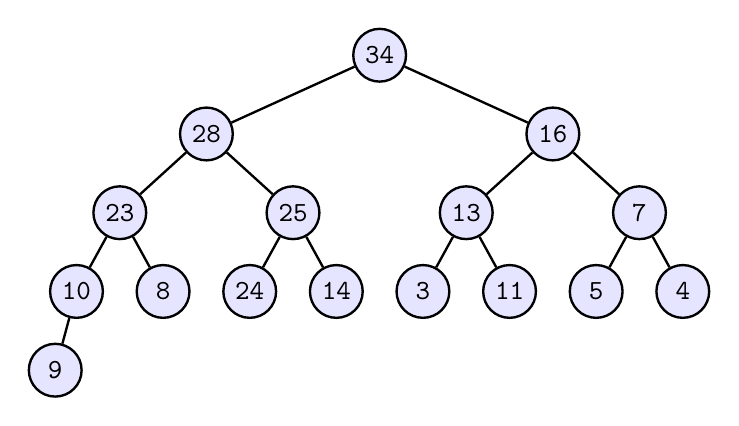
\begin{tikzpicture}

\fill[blue!10] (0.0, 0.0) circle (0.35);
\node [line width=0.03cm,black,minimum size=0.6699999999999999cm,draw,circle] at (0.0,0.0)(34){};\draw (0.0, 0.0) node[color=black] {\texttt{34}};
\fill[blue!10] (-2.2, -1.0) circle (0.35);
\node [line width=0.03cm,black,minimum size=0.6699999999999999cm,draw,circle] at (-2.2,-1.0)(28){};\draw (-2.2, -1.0) node[color=black] {\texttt{28}};
\fill[blue!10] (2.2, -1.0) circle (0.35);
\node [line width=0.03cm,black,minimum size=0.6699999999999999cm,draw,circle] at (2.2,-1.0)(16){};\draw (2.2, -1.0) node[color=black] {\texttt{16}};
\fill[blue!10] (-3.3, -2.0) circle (0.35);
\node [line width=0.03cm,black,minimum size=0.6699999999999999cm,draw,circle] at (-3.3,-2.0)(23){};\draw (-3.3, -2.0) node[color=black] {\texttt{23}};
\fill[blue!10] (-1.1, -2.0) circle (0.35);
\node [line width=0.03cm,black,minimum size=0.6699999999999999cm,draw,circle] at (-1.1,-2.0)(25){};\draw (-1.1, -2.0) node[color=black] {\texttt{25}};
\fill[blue!10] (1.1, -2.0) circle (0.35);
\node [line width=0.03cm,black,minimum size=0.6699999999999999cm,draw,circle] at (1.1,-2.0)(13){};\draw (1.1, -2.0) node[color=black] {\texttt{13}};
\fill[blue!10] (3.3, -2.0) circle (0.35);
\node [line width=0.03cm,black,minimum size=0.6699999999999999cm,draw,circle] at (3.3,-2.0)(7){};\draw (3.3, -2.0) node[color=black] {\texttt{7}};
\fill[blue!10] (-3.85, -3.0) circle (0.35);
\node [line width=0.03cm,black,minimum size=0.6699999999999999cm,draw,circle] at (-3.85,-3.0)(10){};\draw (-3.85, -3.0) node[color=black] {\texttt{10}};
\fill[blue!10] (-2.75, -3.0) circle (0.35);
\node [line width=0.03cm,black,minimum size=0.6699999999999999cm,draw,circle] at (-2.75,-3.0)(8){};\draw (-2.75, -3.0) node[color=black] {\texttt{8}};
\fill[blue!10] (-1.65, -3.0) circle (0.35);
\node [line width=0.03cm,black,minimum size=0.6699999999999999cm,draw,circle] at (-1.65,-3.0)(24){};\draw (-1.65, -3.0) node[color=black] {\texttt{24}};
\fill[blue!10] (-0.55, -3.0) circle (0.35);
\node [line width=0.03cm,black,minimum size=0.6699999999999999cm,draw,circle] at (-0.55,-3.0)(14){};\draw (-0.55, -3.0) node[color=black] {\texttt{14}};
\fill[blue!10] (0.55, -3.0) circle (0.35);
\node [line width=0.03cm,black,minimum size=0.6699999999999999cm,draw,circle] at (0.55,-3.0)(3){};\draw (0.55, -3.0) node[color=black] {\texttt{3}};
\fill[blue!10] (1.65, -3.0) circle (0.35);
\node [line width=0.03cm,black,minimum size=0.6699999999999999cm,draw,circle] at (1.65,-3.0)(11){};\draw (1.65, -3.0) node[color=black] {\texttt{11}};
\fill[blue!10] (2.75, -3.0) circle (0.35);
\node [line width=0.03cm,black,minimum size=0.6699999999999999cm,draw,circle] at (2.75,-3.0)(5){};\draw (2.75, -3.0) node[color=black] {\texttt{5}};
\fill[blue!10] (3.85, -3.0) circle (0.35);
\node [line width=0.03cm,black,minimum size=0.6699999999999999cm,draw,circle] at (3.85,-3.0)(4){};\draw (3.85, -3.0) node[color=black] {\texttt{4}};
\fill[blue!10] (-4.12, -4.0) circle (0.35);
\node [line width=0.03cm,black,minimum size=0.6699999999999999cm,draw,circle] at (-4.12,-4.0)(9){};\draw (-4.12, -4.0) node[color=black] {\texttt{9}};\draw[line width=0.03cm,black] (34) to  (28);
\draw[line width=0.03cm,black] (34) to  (16);
\draw[line width=0.03cm,black] (28) to  (23);
\draw[line width=0.03cm,black] (28) to  (25);
\draw[line width=0.03cm,black] (16) to  (13);
\draw[line width=0.03cm,black] (16) to  (7);
\draw[line width=0.03cm,black] (23) to  (10);
\draw[line width=0.03cm,black] (23) to  (8);
\draw[line width=0.03cm,black] (25) to  (24);
\draw[line width=0.03cm,black] (25) to  (14);
\draw[line width=0.03cm,black] (13) to  (3);
\draw[line width=0.03cm,black] (13) to  (11);
\draw[line width=0.03cm,black] (7) to  (5);
\draw[line width=0.03cm,black] (7) to  (4);
\draw[line width=0.03cm,black] (10) to  (9);
\end{tikzpicture}

\end{center}


\begin{console}[commandchars=\\\{\}]
// move-predecessor-up algorithm
if q is not p->left_:
    q->parent_->right_ = q->left_ 
    p->key_ = q->key_             
    delete q
else:
    \textwhite{p->left_ = q->left}
    \textwhite{p->key_ = q->key_}
    \textwhite{delete q}
\end{console}
After you're done, clean up the algorithm.
Hint: It should look like this:
\begin{console}[commandchars=\\\{\}]
// move-predecessor-up algorithm
if q is not p->left_:
    q->parent_->right_ = q->left_ 
else:
    \textwhite{p->left_ = q->left}
p->key_ = q->key_             
delete q
\end{console}

\end{ex}


\begin{ex}
What if the 8 does not have a left child?
\end{ex}
% The same code works.


\begin{ex}
  What will happen if the node to be deleted has exactly one child?
  For instance the above algorithm assume that \verb!p!
  has a non-NULL left pointer (i.e., \verb!*p! has a left child node).
  But what if \verb!p->left_! is not NULL and
  \verb!p->right_! is NULL?
\end{ex}


The above assume \verb!p->left_! or
\verb!p->right_! is not NULL.
The case left is where both \verb!p->left_!
and \verb!p->right_! are NULL.
This is the case where \verb!*p! is a leave node.
This is easy: we simply remove the node \verb!*p!.
Don't forget, we need to adjust the pointer of \verb!*p!'s parent!
You need to set either the left or the right pointer of
the parent to NULL.
Of course when you arrive at the parent, you wouldn't know
where you came from, whether it's through the left or the right pointer.
No problem ...
\begin{console}
// bst delete leaf
let parent = p->parent_
if parent->left_ is p: // *p is on the left of parent
    parent->left_ = NULL
else
    parent->right_ = NULL
delete p
\end{console}

% This is a general BT algorithm.
% Also, need to handle the case where p is the only node and when
% p is NULL.

\begin{ex}
  \begin{tightlist}
    \li Warning: The above assume that \verb!p! is really pointing to a
    node -- obviously you can't excecute the code when \verb!p! is
    NULL.
    \li Also, if the parent is NULL, the above (obviously) won't work either.
    \li Correct the bst delete leaf algorithm based on the above
    points.
  \end{tightlist}
\end{ex}



\begin{ex}
  Let $T$ be the empty bst (of integers).
  Draw $T$ after each of the following operations:
  \begin{tightlist}
    \li insert 10
    \li insert 15
    \li insert 12
    \li insert 5
    \li insert 0
    \li insert 3
    \li insert 4
    \li insert 9
    \li insert 1
    \li insert 6
    \li delete 10
    \li delete 6
    \li delete 5
    \li delete 12
    \li delete 1
    \li delete 3
    \li delete 4
    \li delete 15
    \li delete 0
  \end{tightlist}
\end{ex}


\textsc{Method 2}.
If copying the key value is more expensive than adjusting pointers,
then the node with 8 can be take the place of the node with value 10, i.e.,
the node with value 10 is deallocate.

\begin{center}
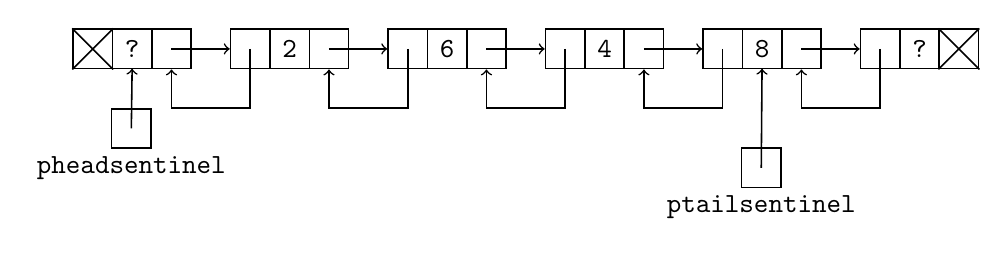
\begin{tikzpicture}

\draw (0.25, 0.25)
  node[draw, line width=0.02cm, , color=black,
       rounded corners=0cm, inner sep=0cm] {

\begin{minipage}[t][0.5cm]{0.5cm}
\mbox{}

\end{minipage}

};\draw (0.25, 0.25) node[color=black] {{\texttt{}}};
\draw (0.75, 0.25)
  node[draw, line width=0.02cm, , color=black,
       rounded corners=0cm, inner sep=0cm] {

\begin{minipage}[t][0.5cm]{0.5cm}
\mbox{}

\end{minipage}

};\draw (0.75, 0.25) node[color=black] {{\texttt{?}}};
\draw (1.25, 0.25)
  node[draw, line width=0.02cm, , color=black,
       rounded corners=0cm, inner sep=0cm] {

\begin{minipage}[t][0.5cm]{0.5cm}
\mbox{}

\end{minipage}

};\draw (1.25, 0.25) node[color=black] {{\texttt{}}};
\draw (2.25, 0.25)
  node[draw, line width=0.02cm, , color=black,
       rounded corners=0cm, inner sep=0cm] {

\begin{minipage}[t][0.5cm]{0.5cm}
\mbox{}

\end{minipage}

};\draw (2.25, 0.25) node[color=black] {{\texttt{}}};
\draw (2.75, 0.25)
  node[draw, line width=0.02cm, , color=black,
       rounded corners=0cm, inner sep=0cm] {

\begin{minipage}[t][0.5cm]{0.5cm}
\mbox{}

\end{minipage}

};\draw (2.75, 0.25) node[color=black] {{\texttt{2}}};
\draw (3.25, 0.25)
  node[draw, line width=0.02cm, , color=black,
       rounded corners=0cm, inner sep=0cm] {

\begin{minipage}[t][0.5cm]{0.5cm}
\mbox{}

\end{minipage}

};\draw (3.25, 0.25) node[color=black] {{\texttt{}}};
\draw (4.25, 0.25)
  node[draw, line width=0.02cm, , color=black,
       rounded corners=0cm, inner sep=0cm] {

\begin{minipage}[t][0.5cm]{0.5cm}
\mbox{}

\end{minipage}

};\draw (4.25, 0.25) node[color=black] {{\texttt{}}};
\draw (4.75, 0.25)
  node[draw, line width=0.02cm, , color=black,
       rounded corners=0cm, inner sep=0cm] {

\begin{minipage}[t][0.5cm]{0.5cm}
\mbox{}

\end{minipage}

};\draw (4.75, 0.25) node[color=black] {{\texttt{6}}};
\draw (5.25, 0.25)
  node[draw, line width=0.02cm, , color=black,
       rounded corners=0cm, inner sep=0cm] {

\begin{minipage}[t][0.5cm]{0.5cm}
\mbox{}

\end{minipage}

};\draw (5.25, 0.25) node[color=black] {{\texttt{}}};
\draw (6.25, 0.25)
  node[draw, line width=0.02cm, , color=black,
       rounded corners=0cm, inner sep=0cm] {

\begin{minipage}[t][0.5cm]{0.5cm}
\mbox{}

\end{minipage}

};\draw (6.25, 0.25) node[color=black] {{\texttt{}}};
\draw (6.75, 0.25)
  node[draw, line width=0.02cm, , color=black,
       rounded corners=0cm, inner sep=0cm] {

\begin{minipage}[t][0.5cm]{0.5cm}
\mbox{}

\end{minipage}

};\draw (6.75, 0.25) node[color=black] {{\texttt{4}}};
\draw (7.25, 0.25)
  node[draw, line width=0.02cm, , color=black,
       rounded corners=0cm, inner sep=0cm] {

\begin{minipage}[t][0.5cm]{0.5cm}
\mbox{}

\end{minipage}

};\draw (7.25, 0.25) node[color=black] {{\texttt{}}};
\draw (8.25, 0.25)
  node[draw, line width=0.02cm, , color=black,
       rounded corners=0cm, inner sep=0cm] {

\begin{minipage}[t][0.5cm]{0.5cm}
\mbox{}

\end{minipage}

};\draw (8.25, 0.25) node[color=black] {{\texttt{}}};
\draw (8.75, 0.25)
  node[draw, line width=0.02cm, , color=black,
       rounded corners=0cm, inner sep=0cm] {

\begin{minipage}[t][0.5cm]{0.5cm}
\mbox{}

\end{minipage}

};\draw (8.75, 0.25) node[color=black] {{\texttt{8}}};
\draw (9.25, 0.25)
  node[draw, line width=0.02cm, , color=black,
       rounded corners=0cm, inner sep=0cm] {

\begin{minipage}[t][0.5cm]{0.5cm}
\mbox{}

\end{minipage}

};\draw (9.25, 0.25) node[color=black] {{\texttt{}}};
\draw (10.25, 0.25)
  node[draw, line width=0.02cm, , color=black,
       rounded corners=0cm, inner sep=0cm] {

\begin{minipage}[t][0.5cm]{0.5cm}
\mbox{}

\end{minipage}

};\draw (10.25, 0.25) node[color=black] {{\texttt{}}};
\draw (10.75, 0.25)
  node[draw, line width=0.02cm, , color=black,
       rounded corners=0cm, inner sep=0cm] {

\begin{minipage}[t][0.5cm]{0.5cm}
\mbox{}

\end{minipage}

};\draw (10.75, 0.25) node[color=black] {{\texttt{?}}};
\draw (11.25, 0.25)
  node[draw, line width=0.02cm, , color=black,
       rounded corners=0cm, inner sep=0cm] {

\begin{minipage}[t][0.5cm]{0.5cm}
\mbox{}

\end{minipage}

};\draw (11.25, 0.25) node[color=black] {{\texttt{}}};\draw[line width=0.02cm,black,->] (1.25,0.25) to  (1.99,0.25);
\draw[line width=0.02cm,black,->] (3.25,0.25) to  (3.99,0.25);
\draw[line width=0.02cm,black,->] (2.25,0.25) to  (2.25,-0.5) to  (1.25,-0.5) to  (1.25,-0.01);
\draw[line width=0.02cm,black,->] (5.25,0.25) to  (5.99,0.25);
\draw[line width=0.02cm,black,->] (4.25,0.25) to  (4.25,-0.5) to  (3.25,-0.5) to  (3.25,-0.01);
\draw[line width=0.02cm,black,->] (7.25,0.25) to  (7.99,0.25);
\draw[line width=0.02cm,black,->] (6.25,0.25) to  (6.25,-0.5) to  (5.25,-0.5) to  (5.25,-0.01);
\draw[line width=0.02cm,black,->] (9.25,0.25) to  (9.99,0.25);
\draw[line width=0.02cm,black,->] (8.25,0.25) to  (8.25,-0.5) to  (7.25,-0.5) to  (7.25,-0.01);
\draw[line width=0.02cm,black,->] (10.25,0.25) to  (10.25,-0.5) to  (9.25,-0.5) to  (9.25,-0.01);
\draw[line width=0.02cm,black] (-0.01,0.51) to  (0.51,-0.01);
\draw[line width=0.02cm,black] (0.51,0.51) to  (-0.01,-0.01);
\draw[line width=0.02cm,black] (10.99,0.51) to  (11.51,-0.01);
\draw[line width=0.02cm,black] (11.51,0.51) to  (10.99,-0.01);

\draw (0.74, -0.76)
  node[draw, line width=0.02cm, , color=black,
       rounded corners=0cm, inner sep=0cm] {

\begin{minipage}[t][0.5cm]{0.5cm}
\mbox{}

\end{minipage}

};\draw (0.74, -0.76) node[color=black] {{\texttt{}}};
\draw (0.74, -1.26)
  node[draw, line width=0.02cm, , color=white,
       rounded corners=0cm, inner sep=0cm] {

\begin{minipage}[t][0.1cm]{0.1cm}
\mbox{}

\end{minipage}

};\draw (0.74, -1.26) node[color=black] {{\texttt{pheadsentinel}}};\draw[line width=0.02cm,black,->] (0.74,-0.76) to  (0.75,0);

\draw (8.74, -1.26)
  node[draw, line width=0.02cm, , color=black,
       rounded corners=0cm, inner sep=0cm] {

\begin{minipage}[t][0.5cm]{0.5cm}
\mbox{}

\end{minipage}

};\draw (8.74, -1.26) node[color=black] {{\texttt{}}};
\draw (8.74, -1.76)
  node[draw, line width=0.02cm, , color=white,
       rounded corners=0cm, inner sep=0cm] {

\begin{minipage}[t][0.1cm]{0.1cm}
\mbox{}

\end{minipage}

};\draw (8.74, -1.76) node[color=black] {{\texttt{ptailsentinel}}};\draw[line width=0.02cm,black,->] (8.74,-1.26) to  (8.75,0);
\end{tikzpicture}

\end{center}


\begin{console}
q->parent_->right_ = q->left_ // point 5 to 6
q->parent_ = p->parent_       // move 8 up to 10 
q->left_ = p->left_
q->right_ = p->right_
delete p
\end{console}

What is the runtime?
Again just like the BST search,
to reach the predessor or successor of the node you are trying to
delete, in the worst case, you have
travel along a path to a leaf.
So again the worst runtime is
\[
O(n)
\]
and again in the average case it's
\[
O(\log n)
\]
since all the above depends on the height of the BST tree.

\begin{console}
ALGORITHM: BST-DELETE
INPUT: node

if node has a left child:
    perform the operation to move the precedessor
    of the node up to the node's position
    and deallocate the appropriate node
else if node has a right child:
    perform the operation to move the sucessor
    of the node to the node's position
    and deallocate the appropriate node
else: // leaf case
    perform bst leaf delete on the node
\end{console}

Don't forget to correct the pseudocode using the exercises and warnings
given.
For instance look at the leaf case: what if the node
does not have a parent -- i.e., the node is in fact the root.


\begin{ex}
Now what if at the node to be deleted, there's exactly one child?
Can you use this information to get a better delete
operation?
For instance notice that in this bst, the node with 0 has a left
child but no right child:
\begin{center}
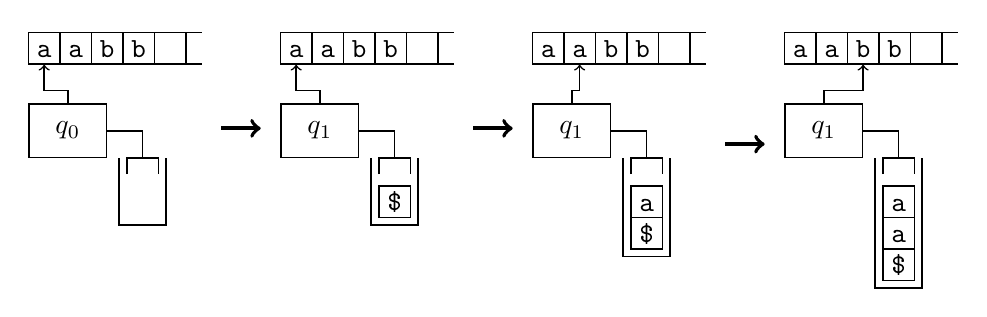
\begin{tikzpicture}

\draw (0.2, 0.2)
  node[draw, line width=0.02cm, , color=black,
       rounded corners=0cm, inner sep=0cm] {

\begin{minipage}[t][0.4cm]{0.4cm}
\mbox{}

\end{minipage}

};\draw (0.2, 0.2) node[color=black] {{\vphantom{aabb\SPACE}\texttt{a}}};
\draw (0.6000000000000001, 0.2)
  node[draw, line width=0.02cm, , color=black,
       rounded corners=0cm, inner sep=0cm] {

\begin{minipage}[t][0.4cm]{0.4cm}
\mbox{}

\end{minipage}

};\draw (0.6000000000000001, 0.2) node[color=black] {{\vphantom{aabb\SPACE}\texttt{a}}};
\draw (1.0, 0.2)
  node[draw, line width=0.02cm, , color=black,
       rounded corners=0cm, inner sep=0cm] {

\begin{minipage}[t][0.4cm]{0.4cm}
\mbox{}

\end{minipage}

};\draw (1.0, 0.2) node[color=black] {{\vphantom{aabb\SPACE}\texttt{b}}};
\draw (1.4000000000000001, 0.2)
  node[draw, line width=0.02cm, , color=black,
       rounded corners=0cm, inner sep=0cm] {

\begin{minipage}[t][0.4cm]{0.4cm}
\mbox{}

\end{minipage}

};\draw (1.4000000000000001, 0.2) node[color=black] {{\vphantom{aabb\SPACE}\texttt{b}}};
\draw (1.7999999999999998, 0.2)
  node[draw, line width=0.02cm, , color=black,
       rounded corners=0cm, inner sep=0cm] {

\begin{minipage}[t][0.4cm]{0.4cm}
\mbox{}

\end{minipage}

};\draw (1.7999999999999998, 0.2) node[color=black] {{\vphantom{aabb\SPACE}\texttt{\SPACE}}};\draw[line width=0.02cm,black] (2.0,0.4) to  (2.2,0.4);
\draw[line width=0.02cm,black] (2.0,0.0) to  (2.2,0.0);

\draw (0.5, -0.85)
  node[draw, line width=0.02cm, , color=black,
       rounded corners=0cm, inner sep=0cm] {

\begin{minipage}[t][0.68cm]{0.98cm}
\mbox{}

\end{minipage}

};\draw (0.5, -0.85) node[color=black] {$q_0$};\draw[line width=0.02cm,black,->] (0.5,-0.5) to  (0.5,-0.34) to  (0.2,-0.34) to  (0.2,-0.01);

\draw (1.45, -1.7499999999999998)
  node[draw=none, line width=0cm, , color=black,
       rounded corners=0cm, inner sep=0cm] {

\begin{minipage}[t][0.4cm]{0.4cm}
\mbox{}

\end{minipage}

};\draw[line width=0.02cm,black] (1.15,-1.2) to  (1.15,-2.05) to  (1.75,-2.05) to  (1.75,-1.2);
\draw[line width=0.02cm,black] (1,-0.85) to  (1.45,-0.85) to  (1.45,-1.2);
\draw[line width=0.02cm,black] (1.25,-1.4) to  (1.25,-1.2) to  (1.65,-1.2) to  (1.65,-1.4);
\draw[line width=0.05cm,black,->] (2.45,-0.82) to  (2.95,-0.82);

\draw (3.4000000000000004, 0.2)
  node[draw, line width=0.02cm, , color=black,
       rounded corners=0cm, inner sep=0cm] {

\begin{minipage}[t][0.4cm]{0.4cm}
\mbox{}

\end{minipage}

};\draw (3.4000000000000004, 0.2) node[color=black] {{\vphantom{\$aabb\SPACE}\texttt{a}}};
\draw (3.8, 0.2)
  node[draw, line width=0.02cm, , color=black,
       rounded corners=0cm, inner sep=0cm] {

\begin{minipage}[t][0.4cm]{0.4cm}
\mbox{}

\end{minipage}

};\draw (3.8, 0.2) node[color=black] {{\vphantom{\$aabb\SPACE}\texttt{a}}};
\draw (4.2, 0.2)
  node[draw, line width=0.02cm, , color=black,
       rounded corners=0cm, inner sep=0cm] {

\begin{minipage}[t][0.4cm]{0.4cm}
\mbox{}

\end{minipage}

};\draw (4.2, 0.2) node[color=black] {{\vphantom{\$aabb\SPACE}\texttt{b}}};
\draw (4.6000000000000005, 0.2)
  node[draw, line width=0.02cm, , color=black,
       rounded corners=0cm, inner sep=0cm] {

\begin{minipage}[t][0.4cm]{0.4cm}
\mbox{}

\end{minipage}

};\draw (4.6000000000000005, 0.2) node[color=black] {{\vphantom{\$aabb\SPACE}\texttt{b}}};
\draw (5.000000000000001, 0.2)
  node[draw, line width=0.02cm, , color=black,
       rounded corners=0cm, inner sep=0cm] {

\begin{minipage}[t][0.4cm]{0.4cm}
\mbox{}

\end{minipage}

};\draw (5.000000000000001, 0.2) node[color=black] {{\vphantom{\$aabb\SPACE}\texttt{\SPACE}}};\draw[line width=0.02cm,black] (5.200000000000001,0.4) to  (5.4,0.4);
\draw[line width=0.02cm,black] (5.200000000000001,0.0) to  (5.4,0.0);

\draw (3.7, -0.85)
  node[draw, line width=0.02cm, , color=black,
       rounded corners=0cm, inner sep=0cm] {

\begin{minipage}[t][0.68cm]{0.98cm}
\mbox{}

\end{minipage}

};\draw (3.7, -0.85) node[color=black] {$q_1$};\draw[line width=0.02cm,black,->] (3.7,-0.5) to  (3.7,-0.34) to  (3.4,-0.34) to  (3.4,-0.01);

\draw (4.65, -1.7499999999999998)
  node[draw, line width=0.02cm, , color=black,
       rounded corners=0cm, inner sep=0cm] {

\begin{minipage}[t][0.4cm]{0.4cm}
\mbox{}

\end{minipage}

};\draw (4.65, -1.7499999999999998) node[color=black] {{\vphantom{\$aabb\SPACE}\texttt{\$}}};\draw[line width=0.02cm,black] (4.35,-1.2) to  (4.35,-2.05) to  (4.95,-2.05) to  (4.95,-1.2);
\draw[line width=0.02cm,black] (4.2,-0.85) to  (4.65,-0.85) to  (4.65,-1.2);
\draw[line width=0.02cm,black] (4.45,-1.4) to  (4.45,-1.2) to  (4.85,-1.2) to  (4.85,-1.4);
\draw[line width=0.05cm,black,->] (5.65,-0.82) to  (6.15,-0.82);

\draw (6.600000000000001, 0.2)
  node[draw, line width=0.02cm, , color=black,
       rounded corners=0cm, inner sep=0cm] {

\begin{minipage}[t][0.4cm]{0.4cm}
\mbox{}

\end{minipage}

};\draw (6.600000000000001, 0.2) node[color=black] {{\vphantom{a\$aabb\SPACE}\texttt{a}}};
\draw (7.000000000000002, 0.2)
  node[draw, line width=0.02cm, , color=black,
       rounded corners=0cm, inner sep=0cm] {

\begin{minipage}[t][0.4cm]{0.4cm}
\mbox{}

\end{minipage}

};\draw (7.000000000000002, 0.2) node[color=black] {{\vphantom{a\$aabb\SPACE}\texttt{a}}};
\draw (7.400000000000002, 0.2)
  node[draw, line width=0.02cm, , color=black,
       rounded corners=0cm, inner sep=0cm] {

\begin{minipage}[t][0.4cm]{0.4cm}
\mbox{}

\end{minipage}

};\draw (7.400000000000002, 0.2) node[color=black] {{\vphantom{a\$aabb\SPACE}\texttt{b}}};
\draw (7.8000000000000025, 0.2)
  node[draw, line width=0.02cm, , color=black,
       rounded corners=0cm, inner sep=0cm] {

\begin{minipage}[t][0.4cm]{0.4cm}
\mbox{}

\end{minipage}

};\draw (7.8000000000000025, 0.2) node[color=black] {{\vphantom{a\$aabb\SPACE}\texttt{b}}};
\draw (8.200000000000003, 0.2)
  node[draw, line width=0.02cm, , color=black,
       rounded corners=0cm, inner sep=0cm] {

\begin{minipage}[t][0.4cm]{0.4cm}
\mbox{}

\end{minipage}

};\draw (8.200000000000003, 0.2) node[color=black] {{\vphantom{a\$aabb\SPACE}\texttt{\SPACE}}};\draw[line width=0.02cm,black] (8.400000000000002,0.4) to  (8.600000000000001,0.4);
\draw[line width=0.02cm,black] (8.400000000000002,0.0) to  (8.600000000000001,0.0);

\draw (6.900000000000001, -0.85)
  node[draw, line width=0.02cm, , color=black,
       rounded corners=0cm, inner sep=0cm] {

\begin{minipage}[t][0.68cm]{0.98cm}
\mbox{}

\end{minipage}

};\draw (6.900000000000001, -0.85) node[color=black] {$q_1$};\draw[line width=0.02cm,black,->] (6.9,-0.5) to  (6.9,-0.34) to  (7.0,-0.34) to  (7.0,-0.01);

\draw (7.850000000000001, -1.7499999999999998)
  node[draw, line width=0.02cm, , color=black,
       rounded corners=0cm, inner sep=0cm] {

\begin{minipage}[t][0.4cm]{0.4cm}
\mbox{}

\end{minipage}

};\draw (7.850000000000001, -1.7499999999999998) node[color=black] {{\vphantom{a\$aabb\SPACE}\texttt{a}}};
\draw (7.850000000000001, -2.1499999999999995)
  node[draw, line width=0.02cm, , color=black,
       rounded corners=0cm, inner sep=0cm] {

\begin{minipage}[t][0.4cm]{0.4cm}
\mbox{}

\end{minipage}

};\draw (7.850000000000001, -2.1499999999999995) node[color=black] {{\vphantom{a\$aabb\SPACE}\texttt{\$}}};\draw[line width=0.02cm,black] (7.55,-1.2) to  (7.55,-2.45) to  (8.15,-2.45) to  (8.15,-1.2);
\draw[line width=0.02cm,black] (7.4,-0.85) to  (7.85,-0.85) to  (7.85,-1.2);
\draw[line width=0.02cm,black] (7.65,-1.4) to  (7.65,-1.2) to  (8.05,-1.2) to  (8.05,-1.4);
\draw[line width=0.05cm,black,->] (8.85,-1.02) to  (9.35,-1.02);

\draw (9.8, 0.2)
  node[draw, line width=0.02cm, , color=black,
       rounded corners=0cm, inner sep=0cm] {

\begin{minipage}[t][0.4cm]{0.4cm}
\mbox{}

\end{minipage}

};\draw (9.8, 0.2) node[color=black] {{\vphantom{aa\$aabb\SPACE}\texttt{a}}};
\draw (10.200000000000003, 0.2)
  node[draw, line width=0.02cm, , color=black,
       rounded corners=0cm, inner sep=0cm] {

\begin{minipage}[t][0.4cm]{0.4cm}
\mbox{}

\end{minipage}

};\draw (10.200000000000003, 0.2) node[color=black] {{\vphantom{aa\$aabb\SPACE}\texttt{a}}};
\draw (10.600000000000001, 0.2)
  node[draw, line width=0.02cm, , color=black,
       rounded corners=0cm, inner sep=0cm] {

\begin{minipage}[t][0.4cm]{0.4cm}
\mbox{}

\end{minipage}

};\draw (10.600000000000001, 0.2) node[color=black] {{\vphantom{aa\$aabb\SPACE}\texttt{b}}};
\draw (11.000000000000004, 0.2)
  node[draw, line width=0.02cm, , color=black,
       rounded corners=0cm, inner sep=0cm] {

\begin{minipage}[t][0.4cm]{0.4cm}
\mbox{}

\end{minipage}

};\draw (11.000000000000004, 0.2) node[color=black] {{\vphantom{aa\$aabb\SPACE}\texttt{b}}};
\draw (11.400000000000002, 0.2)
  node[draw, line width=0.02cm, , color=black,
       rounded corners=0cm, inner sep=0cm] {

\begin{minipage}[t][0.4cm]{0.4cm}
\mbox{}

\end{minipage}

};\draw (11.400000000000002, 0.2) node[color=black] {{\vphantom{aa\$aabb\SPACE}\texttt{\SPACE}}};\draw[line width=0.02cm,black] (11.600000000000003,0.4) to  (11.800000000000002,0.4);
\draw[line width=0.02cm,black] (11.600000000000003,0.0) to  (11.800000000000002,0.0);

\draw (10.100000000000001, -0.85)
  node[draw, line width=0.02cm, , color=black,
       rounded corners=0cm, inner sep=0cm] {

\begin{minipage}[t][0.68cm]{0.98cm}
\mbox{}

\end{minipage}

};\draw (10.100000000000001, -0.85) node[color=black] {$q_1$};\draw[line width=0.02cm,black,->] (10.1,-0.5) to  (10.1,-0.34) to  (10.6,-0.34) to  (10.6,-0.01);

\draw (11.05, -1.7499999999999998)
  node[draw, line width=0.02cm, , color=black,
       rounded corners=0cm, inner sep=0cm] {

\begin{minipage}[t][0.4cm]{0.4cm}
\mbox{}

\end{minipage}

};\draw (11.05, -1.7499999999999998) node[color=black] {{\vphantom{aa\$aabb\SPACE}\texttt{a}}};
\draw (11.05, -2.1499999999999995)
  node[draw, line width=0.02cm, , color=black,
       rounded corners=0cm, inner sep=0cm] {

\begin{minipage}[t][0.4cm]{0.4cm}
\mbox{}

\end{minipage}

};\draw (11.05, -2.1499999999999995) node[color=black] {{\vphantom{aa\$aabb\SPACE}\texttt{a}}};
\draw (11.05, -2.55)
  node[draw, line width=0.02cm, , color=black,
       rounded corners=0cm, inner sep=0cm] {

\begin{minipage}[t][0.4cm]{0.4cm}
\mbox{}

\end{minipage}

};\draw (11.05, -2.55) node[color=black] {{\vphantom{aa\$aabb\SPACE}\texttt{\$}}};\draw[line width=0.02cm,black] (10.75,-1.2) to  (10.75,-2.85) to  (11.35,-2.85) to  (11.35,-1.2);
\draw[line width=0.02cm,black] (10.6,-0.85) to  (11.05,-0.85) to  (11.05,-1.2);
\draw[line width=0.02cm,black] (10.85,-1.4) to  (10.85,-1.2) to  (11.25,-1.2) to  (11.25,-1.4);
\end{tikzpicture}

\end{center}


If you perform the move-predecessor-up, then -1 replaces 0: draw the resulting
picture.
Can you draw another bst diagram that requires fewer changes to the original
bst?
Once you have this algorithm, modify the bst delete algorithm so that
it has this form:
\begin{console}
ALGORITHM: BST-DELETE
INPUT: node

if node has a left child but no right child:
    ...
else if node has a right child but no left child:
    ...
else if node has a right child and a left child:
    ...
else:
    ...
  \end{console}
\end{ex}


\begin{ex}
  \begin{tightlist}
    \li For the case where the node to be deleted has a left and a right child,
    write an algorithm that chooses the predecessor or successor based
    on the greedy approach: choose one that has the shortest depth from the
    node to be deleted.
    \li Is there any reason to choose the longest instead?
    \li Which of the above two is faster?
    \li What about flipping a coin? Why would you want to do that?
    \li How would you modify your BST to include information
    to better decide 
    on whether to move predecessor or sucessor up (instead of just
    tossing a coin)?
  \end{tightlist}
\end{ex}
% Last one: keep left-height and right-height in node. To save a bit more
% just save left-height minus right-height. Note that the update of
% height information is a little more costlier than size. So as an
% approximation, maybe keep leftsize and rightsize. Furthermore storing
% leftsize - rightsize is cheaper too.

\newpage
BST-DELETE algorithm:

Frequently it's convenient to have access to the parent's child point
that points to \verb!p!.
For instance if \verb!*p! is the right child or the parent
\verb!*(p->parent_)!, then it's convenient to have a function
to return a reference to \verb!p->parent_->right_!.
This can be used for any binary tree (not just bst).
This can be easily generalize to any tree.
\begin{console}
ALGORITHM: PARENT-CHILD-POINTER
INPUT:  p
RETURN: reference to left_ or right_ of *(p->parent)

let parent = p->parent_
if parent == NULL:
    return NULL // *p is root
else:
    if parent->left_ is p:
        return parent->left_ (by reference)
    else:
        return parent->right_
\end{console}

The following deletes the node \verb!*p! assuming that it's a leaf.
This can be easily generalized for any tree.
\begin{console}
ALGORITHM: LEAF-DELETE
INPUT: proot
       p

if *p is root:
    proot = NULL
else:
    PARENT-CHILD-POINTER(p) = NULL
delete p
\end{console}
(This is a general algorithm for binary trees, not just BST.)

The following cuts out a node $n$
directly from the tree so that the parent of $n$ is joined to
either the left or right child of $n$.
For instance if you perform punch through at 0 in the left direction.
It is also assumed that \verb!p! is not NULL and
\verb!p->parent_! is not NULL.
\begin{center}
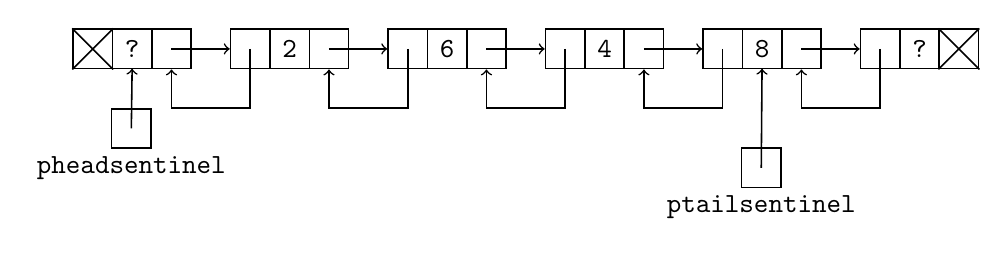
\begin{tikzpicture}

\draw (0.25, 0.25)
  node[draw, line width=0.02cm, , color=black,
       rounded corners=0cm, inner sep=0cm] {

\begin{minipage}[t][0.5cm]{0.5cm}
\mbox{}

\end{minipage}

};\draw (0.25, 0.25) node[color=black] {{\texttt{}}};
\draw (0.75, 0.25)
  node[draw, line width=0.02cm, , color=black,
       rounded corners=0cm, inner sep=0cm] {

\begin{minipage}[t][0.5cm]{0.5cm}
\mbox{}

\end{minipage}

};\draw (0.75, 0.25) node[color=black] {{\texttt{?}}};
\draw (1.25, 0.25)
  node[draw, line width=0.02cm, , color=black,
       rounded corners=0cm, inner sep=0cm] {

\begin{minipage}[t][0.5cm]{0.5cm}
\mbox{}

\end{minipage}

};\draw (1.25, 0.25) node[color=black] {{\texttt{}}};
\draw (2.25, 0.25)
  node[draw, line width=0.02cm, , color=black,
       rounded corners=0cm, inner sep=0cm] {

\begin{minipage}[t][0.5cm]{0.5cm}
\mbox{}

\end{minipage}

};\draw (2.25, 0.25) node[color=black] {{\texttt{}}};
\draw (2.75, 0.25)
  node[draw, line width=0.02cm, , color=black,
       rounded corners=0cm, inner sep=0cm] {

\begin{minipage}[t][0.5cm]{0.5cm}
\mbox{}

\end{minipage}

};\draw (2.75, 0.25) node[color=black] {{\texttt{2}}};
\draw (3.25, 0.25)
  node[draw, line width=0.02cm, , color=black,
       rounded corners=0cm, inner sep=0cm] {

\begin{minipage}[t][0.5cm]{0.5cm}
\mbox{}

\end{minipage}

};\draw (3.25, 0.25) node[color=black] {{\texttt{}}};
\draw (4.25, 0.25)
  node[draw, line width=0.02cm, , color=black,
       rounded corners=0cm, inner sep=0cm] {

\begin{minipage}[t][0.5cm]{0.5cm}
\mbox{}

\end{minipage}

};\draw (4.25, 0.25) node[color=black] {{\texttt{}}};
\draw (4.75, 0.25)
  node[draw, line width=0.02cm, , color=black,
       rounded corners=0cm, inner sep=0cm] {

\begin{minipage}[t][0.5cm]{0.5cm}
\mbox{}

\end{minipage}

};\draw (4.75, 0.25) node[color=black] {{\texttt{6}}};
\draw (5.25, 0.25)
  node[draw, line width=0.02cm, , color=black,
       rounded corners=0cm, inner sep=0cm] {

\begin{minipage}[t][0.5cm]{0.5cm}
\mbox{}

\end{minipage}

};\draw (5.25, 0.25) node[color=black] {{\texttt{}}};
\draw (6.25, 0.25)
  node[draw, line width=0.02cm, , color=black,
       rounded corners=0cm, inner sep=0cm] {

\begin{minipage}[t][0.5cm]{0.5cm}
\mbox{}

\end{minipage}

};\draw (6.25, 0.25) node[color=black] {{\texttt{}}};
\draw (6.75, 0.25)
  node[draw, line width=0.02cm, , color=black,
       rounded corners=0cm, inner sep=0cm] {

\begin{minipage}[t][0.5cm]{0.5cm}
\mbox{}

\end{minipage}

};\draw (6.75, 0.25) node[color=black] {{\texttt{4}}};
\draw (7.25, 0.25)
  node[draw, line width=0.02cm, , color=black,
       rounded corners=0cm, inner sep=0cm] {

\begin{minipage}[t][0.5cm]{0.5cm}
\mbox{}

\end{minipage}

};\draw (7.25, 0.25) node[color=black] {{\texttt{}}};
\draw (8.25, 0.25)
  node[draw, line width=0.02cm, , color=black,
       rounded corners=0cm, inner sep=0cm] {

\begin{minipage}[t][0.5cm]{0.5cm}
\mbox{}

\end{minipage}

};\draw (8.25, 0.25) node[color=black] {{\texttt{}}};
\draw (8.75, 0.25)
  node[draw, line width=0.02cm, , color=black,
       rounded corners=0cm, inner sep=0cm] {

\begin{minipage}[t][0.5cm]{0.5cm}
\mbox{}

\end{minipage}

};\draw (8.75, 0.25) node[color=black] {{\texttt{8}}};
\draw (9.25, 0.25)
  node[draw, line width=0.02cm, , color=black,
       rounded corners=0cm, inner sep=0cm] {

\begin{minipage}[t][0.5cm]{0.5cm}
\mbox{}

\end{minipage}

};\draw (9.25, 0.25) node[color=black] {{\texttt{}}};
\draw (10.25, 0.25)
  node[draw, line width=0.02cm, , color=black,
       rounded corners=0cm, inner sep=0cm] {

\begin{minipage}[t][0.5cm]{0.5cm}
\mbox{}

\end{minipage}

};\draw (10.25, 0.25) node[color=black] {{\texttt{}}};
\draw (10.75, 0.25)
  node[draw, line width=0.02cm, , color=black,
       rounded corners=0cm, inner sep=0cm] {

\begin{minipage}[t][0.5cm]{0.5cm}
\mbox{}

\end{minipage}

};\draw (10.75, 0.25) node[color=black] {{\texttt{?}}};
\draw (11.25, 0.25)
  node[draw, line width=0.02cm, , color=black,
       rounded corners=0cm, inner sep=0cm] {

\begin{minipage}[t][0.5cm]{0.5cm}
\mbox{}

\end{minipage}

};\draw (11.25, 0.25) node[color=black] {{\texttt{}}};\draw[line width=0.02cm,black,->] (1.25,0.25) to  (1.99,0.25);
\draw[line width=0.02cm,black,->] (3.25,0.25) to  (3.99,0.25);
\draw[line width=0.02cm,black,->] (2.25,0.25) to  (2.25,-0.5) to  (1.25,-0.5) to  (1.25,-0.01);
\draw[line width=0.02cm,black,->] (5.25,0.25) to  (5.99,0.25);
\draw[line width=0.02cm,black,->] (4.25,0.25) to  (4.25,-0.5) to  (3.25,-0.5) to  (3.25,-0.01);
\draw[line width=0.02cm,black,->] (7.25,0.25) to  (7.99,0.25);
\draw[line width=0.02cm,black,->] (6.25,0.25) to  (6.25,-0.5) to  (5.25,-0.5) to  (5.25,-0.01);
\draw[line width=0.02cm,black,->] (9.25,0.25) to  (9.99,0.25);
\draw[line width=0.02cm,black,->] (8.25,0.25) to  (8.25,-0.5) to  (7.25,-0.5) to  (7.25,-0.01);
\draw[line width=0.02cm,black,->] (10.25,0.25) to  (10.25,-0.5) to  (9.25,-0.5) to  (9.25,-0.01);
\draw[line width=0.02cm,black] (-0.01,0.51) to  (0.51,-0.01);
\draw[line width=0.02cm,black] (0.51,0.51) to  (-0.01,-0.01);
\draw[line width=0.02cm,black] (10.99,0.51) to  (11.51,-0.01);
\draw[line width=0.02cm,black] (11.51,0.51) to  (10.99,-0.01);

\draw (0.74, -0.76)
  node[draw, line width=0.02cm, , color=black,
       rounded corners=0cm, inner sep=0cm] {

\begin{minipage}[t][0.5cm]{0.5cm}
\mbox{}

\end{minipage}

};\draw (0.74, -0.76) node[color=black] {{\texttt{}}};
\draw (0.74, -1.26)
  node[draw, line width=0.02cm, , color=white,
       rounded corners=0cm, inner sep=0cm] {

\begin{minipage}[t][0.1cm]{0.1cm}
\mbox{}

\end{minipage}

};\draw (0.74, -1.26) node[color=black] {{\texttt{pheadsentinel}}};\draw[line width=0.02cm,black,->] (0.74,-0.76) to  (0.75,0);

\draw (8.74, -1.26)
  node[draw, line width=0.02cm, , color=black,
       rounded corners=0cm, inner sep=0cm] {

\begin{minipage}[t][0.5cm]{0.5cm}
\mbox{}

\end{minipage}

};\draw (8.74, -1.26) node[color=black] {{\texttt{}}};
\draw (8.74, -1.76)
  node[draw, line width=0.02cm, , color=white,
       rounded corners=0cm, inner sep=0cm] {

\begin{minipage}[t][0.1cm]{0.1cm}
\mbox{}

\end{minipage}

};\draw (8.74, -1.76) node[color=black] {{\texttt{ptailsentinel}}};\draw[line width=0.02cm,black,->] (8.74,-1.26) to  (8.75,0);
\end{tikzpicture}

\end{center}


we get
\begin{center}
\begin{tikzpicture}

\fill[white] (11.0, 0.0) circle (0.3);
\node [line width=0.03cm,black,minimum size=0.57cm,draw,circle] at (11.0,0.0)(A){};\draw (11.0, 0.0) node[color=black] {\texttt{20}};
\fill[white] (10.0, -0.7) circle (0.3);
\node [line width=0.03cm,black,minimum size=0.57cm,draw,circle] at (10.0,-0.7)(a){};\draw (10.0, -0.7) node[color=black] {\texttt{10}};
\fill[white] (8.0, -2.1) circle (0.3);
\node [line width=0.03cm,black,minimum size=0.57cm,draw,circle] at (8.0,-2.1)(e){};\draw (8.0, -2.1) node[color=black] {\texttt{-2}};
\fill[white] (7.0, -2.8) circle (0.3);
\node [line width=0.03cm,black,minimum size=0.57cm,draw,circle] at (7.0,-2.8)(k){};\draw (7.0, -2.8) node[color=black] {\texttt{-3}};
\fill[white] (9.0, -2.8) circle (0.3);
\node [line width=0.03cm,black,minimum size=0.57cm,draw,circle] at (9.0,-2.8)(l){};\draw (9.0, -2.8) node[color=black] {\texttt{-1}};
\fill[white] (11.0, -1.4) circle (0.3);
\node [line width=0.03cm,black,minimum size=0.57cm,draw,circle] at (11.0,-1.4)(p){};\draw (11.0, -1.4) node[color=black] {\texttt{15}};\draw[line width=0.03cm,black,->,>=triangle 60] (A) to  (a);
\draw[line width=0.03cm,black,->,>=triangle 60] (a) to  (p);
\draw[line width=0.03cm,black,->,>=triangle 60] (a) to  (e);
\draw[line width=0.03cm,black,->,>=triangle 60] (e) to  (k);
\draw[line width=0.03cm,black,->,>=triangle 60] (e) to  (l);
\end{tikzpicture}

\end{center}

\begin{center}
\begin{tikzpicture}

\fill[white] (11.0, 0.0) circle (0.3);
\node [line width=0.03cm,black,minimum size=0.57cm,draw,circle] at (11.0,0.0)(A){};\draw (11.0, 0.0) node[color=black] {\texttt{20}};
\fill[white] (10.0, -0.7) circle (0.3);
\node [line width=0.03cm,black,minimum size=0.57cm,draw,circle] at (10.0,-0.7)(a){};\draw (10.0, -0.7) node[color=black] {\texttt{10}};
\fill[white] (9.0, -1.4) circle (0.3);
\node [line width=0.03cm,black,minimum size=0.57cm,draw,circle] at (9.0,-1.4)(b){};\draw (9.0, -1.4) node[color=black] {\texttt{0}};
\fill[white] (8.0, -2.1) circle (0.3);
\node [line width=0.03cm,black,minimum size=0.57cm,draw,circle] at (8.0,-2.1)(e){};\draw (8.0, -2.1) node[color=black] {\texttt{-2}};
\fill[white] (7.0, -2.8) circle (0.3);
\node [line width=0.03cm,black,minimum size=0.57cm,draw,circle] at (7.0,-2.8)(k){};\draw (7.0, -2.8) node[color=black] {\texttt{-3}};
\fill[white] (9.0, -2.8) circle (0.3);
\node [line width=0.03cm,black,minimum size=0.57cm,draw,circle] at (9.0,-2.8)(l){};\draw (9.0, -2.8) node[color=black] {\texttt{-1}};
\fill[white] (11.0, -1.4) circle (0.3);
\node [line width=0.03cm,black,minimum size=0.57cm,draw,circle] at (11.0,-1.4)(p){};\draw (11.0, -1.4) node[color=black] {\texttt{15}};\draw[line width=0.03cm,black,->,>=triangle 60] (A) to  (a);
\draw[line width=0.03cm,black,->,>=triangle 60] (a) to  (p);
\draw[line width=0.03cm,black,->,>=triangle 60] (a) to  (b);
\draw[line width=0.03cm,black,->,>=triangle 60] (b) to  (e);
\draw[line width=0.03cm,black,->,>=triangle 60] (e) to  (k);
\draw[line width=0.03cm,black,->,>=triangle 60] (e) to  (l);
\end{tikzpicture}

\end{center}


The algorithm deallocates the node that is punched through
but does not deallocate subtrees. For instance in the above
it's assumed that 0 does not have any right subtree to deallocate.
It allows \verb!p->parent_! to be NULL. In that case
a child of \verb!*p! becomes the root.
For instance if we punch through at 20 in the left direction for
the following tree
\begin{center}
\begin{tikzpicture}

\fill[white] (11.0, 0.0) circle (0.3);
\node [line width=0.03cm,black,minimum size=0.57cm,draw,circle] at (11.0,0.0)(A){};\draw (11.0, 0.0) node[color=black] {\texttt{20}};
\fill[white] (10.0, -0.7) circle (0.3);
\node [line width=0.03cm,black,minimum size=0.57cm,draw,circle] at (10.0,-0.7)(a){};\draw (10.0, -0.7) node[color=black] {\texttt{10}};
\fill[white] (9.0, -1.4) circle (0.3);
\node [line width=0.03cm,black,minimum size=0.57cm,draw,circle] at (9.0,-1.4)(b){};\draw (9.0, -1.4) node[color=black] {\texttt{0}};
\fill[white] (8.0, -2.1) circle (0.3);
\node [line width=0.03cm,black,minimum size=0.57cm,draw,circle] at (8.0,-2.1)(e){};\draw (8.0, -2.1) node[color=black] {\texttt{-2}};
\fill[white] (7.0, -2.8) circle (0.3);
\node [line width=0.03cm,black,minimum size=0.57cm,draw,circle] at (7.0,-2.8)(k){};\draw (7.0, -2.8) node[color=black] {\texttt{-3}};
\fill[white] (9.0, -2.8) circle (0.3);
\node [line width=0.03cm,black,minimum size=0.57cm,draw,circle] at (9.0,-2.8)(l){};\draw (9.0, -2.8) node[color=black] {\texttt{-1}};
\fill[white] (11.0, -1.4) circle (0.3);
\node [line width=0.03cm,black,minimum size=0.57cm,draw,circle] at (11.0,-1.4)(p){};\draw (11.0, -1.4) node[color=black] {\texttt{15}};\draw[line width=0.03cm,black,->,>=triangle 60] (A) to  (a);
\draw[line width=0.03cm,black,->,>=triangle 60] (a) to  (p);
\draw[line width=0.03cm,black,->,>=triangle 60] (a) to  (b);
\draw[line width=0.03cm,black,->,>=triangle 60] (b) to  (e);
\draw[line width=0.03cm,black,->,>=triangle 60] (e) to  (k);
\draw[line width=0.03cm,black,->,>=triangle 60] (e) to  (l);
\end{tikzpicture}

\end{center}


we get
\begin{center}
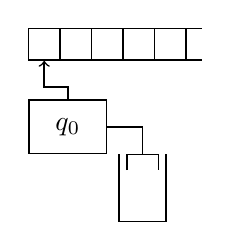
\begin{tikzpicture}

\draw (0.2, 0.2)
  node[draw, line width=0.02cm, , color=black,
       rounded corners=0cm, inner sep=0cm] {

\begin{minipage}[t][0.4cm]{0.4cm}
\mbox{}

\end{minipage}

};\draw (0.2, 0.2) node[color=black] {{\vphantom{\SPACE\SPACE\SPACE\SPACE\SPACE}\texttt{\SPACE}}};
\draw (0.6000000000000001, 0.2)
  node[draw, line width=0.02cm, , color=black,
       rounded corners=0cm, inner sep=0cm] {

\begin{minipage}[t][0.4cm]{0.4cm}
\mbox{}

\end{minipage}

};\draw (0.6000000000000001, 0.2) node[color=black] {{\vphantom{\SPACE\SPACE\SPACE\SPACE\SPACE}\texttt{\SPACE}}};
\draw (1.0, 0.2)
  node[draw, line width=0.02cm, , color=black,
       rounded corners=0cm, inner sep=0cm] {

\begin{minipage}[t][0.4cm]{0.4cm}
\mbox{}

\end{minipage}

};\draw (1.0, 0.2) node[color=black] {{\vphantom{\SPACE\SPACE\SPACE\SPACE\SPACE}\texttt{\SPACE}}};
\draw (1.4000000000000001, 0.2)
  node[draw, line width=0.02cm, , color=black,
       rounded corners=0cm, inner sep=0cm] {

\begin{minipage}[t][0.4cm]{0.4cm}
\mbox{}

\end{minipage}

};\draw (1.4000000000000001, 0.2) node[color=black] {{\vphantom{\SPACE\SPACE\SPACE\SPACE\SPACE}\texttt{\SPACE}}};
\draw (1.7999999999999998, 0.2)
  node[draw, line width=0.02cm, , color=black,
       rounded corners=0cm, inner sep=0cm] {

\begin{minipage}[t][0.4cm]{0.4cm}
\mbox{}

\end{minipage}

};\draw (1.7999999999999998, 0.2) node[color=black] {{\vphantom{\SPACE\SPACE\SPACE\SPACE\SPACE}\texttt{\SPACE}}};\draw[line width=0.02cm,black] (2.0,0.4) to  (2.2,0.4);
\draw[line width=0.02cm,black] (2.0,0.0) to  (2.2,0.0);

\draw (0.5, -0.85)
  node[draw, line width=0.02cm, , color=black,
       rounded corners=0cm, inner sep=0cm] {

\begin{minipage}[t][0.68cm]{0.98cm}
\mbox{}

\end{minipage}

};\draw (0.5, -0.85) node[color=black] {$q_0$};\draw[line width=0.02cm,black,->] (0.5,-0.5) to  (0.5,-0.34) to  (0.2,-0.34) to  (0.2,-0.01);

\draw (1.45, -1.7499999999999998)
  node[draw=none, line width=0cm, , color=black,
       rounded corners=0cm, inner sep=0cm] {

\begin{minipage}[t][0.4cm]{0.4cm}
\mbox{}

\end{minipage}

};\draw[line width=0.02cm,black] (1.15,-1.2) to  (1.15,-2.05) to  (1.75,-2.05) to  (1.75,-1.2);
\draw[line width=0.02cm,black] (1,-0.85) to  (1.45,-0.85) to  (1.45,-1.2);
\draw[line width=0.02cm,black] (1.25,-1.4) to  (1.25,-1.2) to  (1.65,-1.2) to  (1.65,-1.4);
\end{tikzpicture}

\end{center}



We can also punch through a node and go to the right.
For instance in the following,
\begin{center}
\begin{tikzpicture}

\fill[white] (11.0, 0.0) circle (0.3);
\node [line width=0.03cm,black,minimum size=0.57cm,draw,circle] at (11.0,0.0)(A){};\draw (11.0, 0.0) node[color=black] {\texttt{20}};
\fill[white] (10.0, -0.7) circle (0.3);
\node [line width=0.03cm,black,minimum size=0.57cm,draw,circle] at (10.0,-0.7)(a){};\draw (10.0, -0.7) node[color=black] {\texttt{10}};
\fill[white] (9.0, -1.4) circle (0.3);
\node [line width=0.03cm,black,minimum size=0.57cm,draw,circle] at (9.0,-1.4)(b){};\draw (9.0, -1.4) node[color=black] {\texttt{5}};
\fill[white] (10.0, -2.1) circle (0.3);
\node [line width=0.03cm,black,minimum size=0.57cm,draw,circle] at (10.0,-2.1)(e){};\draw (10.0, -2.1) node[color=black] {\texttt{8}};
\fill[white] (9.0, -2.8) circle (0.3);
\node [line width=0.03cm,black,minimum size=0.57cm,draw,circle] at (9.0,-2.8)(k){};\draw (9.0, -2.8) node[color=black] {\texttt{6}};
\fill[white] (11.0, -2.8) circle (0.3);
\node [line width=0.03cm,black,minimum size=0.57cm,draw,circle] at (11.0,-2.8)(l){};\draw (11.0, -2.8) node[color=black] {\texttt{9}};
\fill[white] (11.0, -1.4) circle (0.3);
\node [line width=0.03cm,black,minimum size=0.57cm,draw,circle] at (11.0,-1.4)(p){};\draw (11.0, -1.4) node[color=black] {\texttt{15}};\draw[line width=0.03cm,black,->,>=triangle 60] (A) to  (a);
\draw[line width=0.03cm,black,->,>=triangle 60] (a) to  (p);
\draw[line width=0.03cm,black,->,>=triangle 60] (a) to  (b);
\draw[line width=0.03cm,black,->,>=triangle 60] (b) to  (e);
\draw[line width=0.03cm,black,->,>=triangle 60] (e) to  (k);
\draw[line width=0.03cm,black,->,>=triangle 60] (e) to  (l);
\end{tikzpicture}

\end{center}


we can remove 5 by punching
through at 5 and go to the right to get this:
\begin{center}
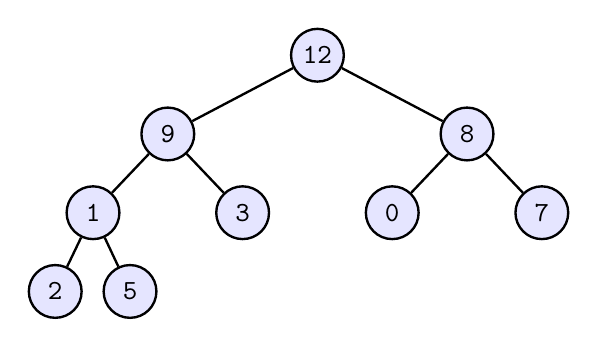
\begin{tikzpicture}

\fill[blue!10] (0.0, 0.0) circle (0.35);
\node [line width=0.03cm,black,minimum size=0.6699999999999999cm,draw,circle] at (0.0,0.0)(12){};\draw (0.0, 0.0) node[color=black] {\texttt{12}};
\fill[blue!10] (-1.9, -1.0) circle (0.35);
\node [line width=0.03cm,black,minimum size=0.6699999999999999cm,draw,circle] at (-1.9,-1.0)(9){};\draw (-1.9, -1.0) node[color=black] {\texttt{9}};
\fill[blue!10] (1.9, -1.0) circle (0.35);
\node [line width=0.03cm,black,minimum size=0.6699999999999999cm,draw,circle] at (1.9,-1.0)(8){};\draw (1.9, -1.0) node[color=black] {\texttt{8}};
\fill[blue!10] (-2.85, -2.0) circle (0.35);
\node [line width=0.03cm,black,minimum size=0.6699999999999999cm,draw,circle] at (-2.85,-2.0)(1){};\draw (-2.85, -2.0) node[color=black] {\texttt{1}};
\fill[blue!10] (-0.95, -2.0) circle (0.35);
\node [line width=0.03cm,black,minimum size=0.6699999999999999cm,draw,circle] at (-0.95,-2.0)(3){};\draw (-0.95, -2.0) node[color=black] {\texttt{3}};
\fill[blue!10] (0.95, -2.0) circle (0.35);
\node [line width=0.03cm,black,minimum size=0.6699999999999999cm,draw,circle] at (0.95,-2.0)(0){};\draw (0.95, -2.0) node[color=black] {\texttt{0}};
\fill[blue!10] (2.85, -2.0) circle (0.35);
\node [line width=0.03cm,black,minimum size=0.6699999999999999cm,draw,circle] at (2.85,-2.0)(7){};\draw (2.85, -2.0) node[color=black] {\texttt{7}};
\fill[blue!10] (-3.33, -3.0) circle (0.35);
\node [line width=0.03cm,black,minimum size=0.6699999999999999cm,draw,circle] at (-3.33,-3.0)(2){};\draw (-3.33, -3.0) node[color=black] {\texttt{2}};
\fill[blue!10] (-2.38, -3.0) circle (0.35);
\node [line width=0.03cm,black,minimum size=0.6699999999999999cm,draw,circle] at (-2.38,-3.0)(5){};\draw (-2.38, -3.0) node[color=black] {\texttt{5}};\draw[line width=0.03cm,black] (12) to  (9);
\draw[line width=0.03cm,black] (12) to  (8);
\draw[line width=0.03cm,black] (9) to  (1);
\draw[line width=0.03cm,black] (9) to  (3);
\draw[line width=0.03cm,black] (8) to  (0);
\draw[line width=0.03cm,black] (8) to  (7);
\draw[line width=0.03cm,black] (1) to  (2);
\draw[line width=0.03cm,black] (1) to  (5);
\end{tikzpicture}

\end{center}


Here are the two algorithms for punch-through delete:
\begin{console}
ALGORITHM: PUNCH-THROUGH-TO-LEFT
INPUT: proot
       p

if p->parent is NULL:
    proot = p->left_
else:
    p->parent->left_ = p->left_
delete p
\end{console}
\begin{console}
ALGORITHM: PUNCH-THROUGH-TO-RIGHT
INPUT: proot
       p

if p->parent is NULL:
    proot = r->right_
else:
    p->parent->right_ = p->right_
delete p
\end{console}

This is the version without the punch-through deletion:
{\small
\begin{console}
ALGORITHM: BST-DELETE
INPUT: proot
       p

if p->left_ is NULL:
    if p->right_ is NULL:
        BST-DELETE-LEAF(proot, p)
    else:
        BST-MOVE-SUCC-UP(proot, p)
else:
    if p->right_ is NULL:
        BST-MOVE-PRED-UP(proot, p)
    else:
        # two children case
        if rand() % 2 == 0:
            BST-MOVE-PRED-UP(proot, p)
        else:
            BST-MOVE-SUCC-UP(proot, p)
\end{console}
}
This one uses the punch-through:
{\small
\begin{console}
ALGORITHM: BST-DELETE
INPUT: proot
       p

if p->left_ is NULL:
    if p->right_ is NULL:
        BST-DELETE-LEAF(proot, p)
    else:
        PUNCH-THROUGH-TO-RIGHT(proot, p)
else:
    if p_->right_ is NULL:
        PUNCH-THROUGH-TO-LEFT(proot, p)
    else:
        # two children case
        if rand() % 2 is 0:
            BST-MOVE-PRED-UP(proot, p)
        else:
            BST-MOVE-SUCC-UP(proot, p)
\end{console}
}

% To generalize, need to have some way of telling the path to the root
% for instance p should contain the pointers of ancestors back to root
% a recursive function contains only aancestor chain of nodes but not the
% point use to move down
% maybe nodes should contain reference/pointer to the parent's pointer
% leading to the node
% Call this the parent_child_ptr the pointer in *(p->parent) that points
% to p
% To delete *p from parent do
%     *(p->parent_child_ptr_) = NULL
%     delete p
% If this is not kept in the node, then can also keep inside an iterator
% Maybe an iterator should contain
% - pointer to node
% - pointer to parent (in case node does not have parent pointer)
% - pointer to pointer in parent that points to node
% For recusive functions, maybe should write them like this:
%
% void f(p):
%     if p == null:
%         return
%     else:
%         Node ** child_pointer
%         if ...
%             child_pointer = &(p->left_)
%             f(p->left_)
%         else:
%             child_pointer = &(p->right_)
%             f(p->right_)
%
%         do some more computation on *p possibly using
%         parent_child_pointer



\newpage
\begin{ex}
  Write a function
\begin{console}
bool is_bst(Node * p);
\end{console}
that checks if the binary tree at \verb!p! is a BST.
\end{ex}



\newpage
\begin{ex}
  Suppose you're given an array of integers which is already
  sorted in ascending order.
  How would your construct a BST with the values in this array
  so that the height of the tree is as small as possible?
\end{ex}
% build(arr, start=0, end=n-1, p)
%    if start >= end:
%        return NULL
%    else
%        mid = (start + end) / 2
%        leftroot = build(arr, start, m-id - 1)
%        rightroot = build(arr, mid + 1, end)
%        p = new Node(mid)   
%        p->left_ = leftroot
%        p->right_ = rightroot
% -- note that this is postorder except that the tree does not
%    exist yet. So technically not a traversal



\newpage
\begin{ex}
  Range search:
  Let $a < b$ and $T$ be a BST.
  \begin{itemize}
    \li Write a function that returns true if there is a key
    $k$ such that $a \leq k < b$.
    \li Write a function that returns a pointer
    that points to the node in $T$
    with the smallest key $k$ such that
    $a \leq k < b$.
    If there is none, NULL is returned.
    \li Write a function that accepts a pointer $p$,
    and a value $b$ and that returns a pointer
    that points to the node in $T$
    with the smallest key $k$ such that
    \verb!p->key_! $< k < b$.
    If there is none, NULL is returned.
    
    \li Write a function that returns a vector or list of pointers
    pointing to all nodes in $T$ with values in $[a, b)$.
    The pointers must be arranged in order of the key values of their
    nodes.

    \li Write an iterator class so that that does the same as
    the above. For instance \verb!BST_iterator p(proot, a, b)!
    will create the iterator and you iterate through all the
    pointers of the required nodes by doing
    {\small
    \begin{Verbatim}[frame=single]
while (p != NULL)
{
    std::cout << p->key() << '\n';
    ++p;
}
    \end{Verbatim}
    }
  \end{itemize}
\end{ex}

  
\newpage
\subsection{Comparing BST and sorted array}

I hope that you see that the BST search if the tree is balanced (i.e.,
roughyl equal number of nodes on the left and right for each node),
the nodes that you visit is similar to the values you would
visit in a sorted array with the same values.

Here's our first BST again:

\begin{center}
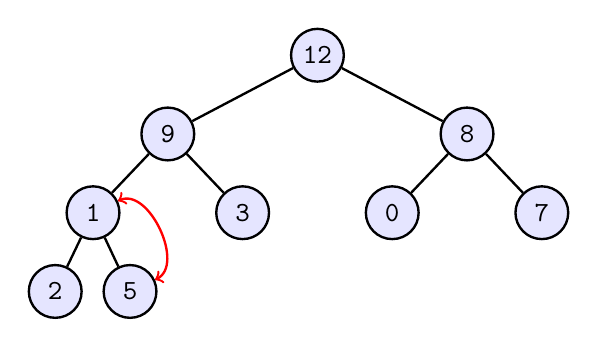
\begin{tikzpicture}

\fill[blue!10] (0.0, 0.0) circle (0.35);
\node [line width=0.03cm,black,minimum size=0.6699999999999999cm,draw,circle] at (0.0,0.0)(12){};\draw (0.0, 0.0) node[color=black] {\texttt{12}};
\fill[blue!10] (-1.9, -1.0) circle (0.35);
\node [line width=0.03cm,black,minimum size=0.6699999999999999cm,draw,circle] at (-1.9,-1.0)(9){};\draw (-1.9, -1.0) node[color=black] {\texttt{9}};
\fill[blue!10] (1.9, -1.0) circle (0.35);
\node [line width=0.03cm,black,minimum size=0.6699999999999999cm,draw,circle] at (1.9,-1.0)(8){};\draw (1.9, -1.0) node[color=black] {\texttt{8}};
\fill[blue!10] (-2.85, -2.0) circle (0.35);
\node [line width=0.03cm,black,minimum size=0.6699999999999999cm,draw,circle] at (-2.85,-2.0)(1){};\draw (-2.85, -2.0) node[color=black] {\texttt{1}};
\fill[blue!10] (-0.95, -2.0) circle (0.35);
\node [line width=0.03cm,black,minimum size=0.6699999999999999cm,draw,circle] at (-0.95,-2.0)(3){};\draw (-0.95, -2.0) node[color=black] {\texttt{3}};
\fill[blue!10] (0.95, -2.0) circle (0.35);
\node [line width=0.03cm,black,minimum size=0.6699999999999999cm,draw,circle] at (0.95,-2.0)(0){};\draw (0.95, -2.0) node[color=black] {\texttt{0}};
\fill[blue!10] (2.85, -2.0) circle (0.35);
\node [line width=0.03cm,black,minimum size=0.6699999999999999cm,draw,circle] at (2.85,-2.0)(7){};\draw (2.85, -2.0) node[color=black] {\texttt{7}};
\fill[blue!10] (-3.33, -3.0) circle (0.35);
\node [line width=0.03cm,black,minimum size=0.6699999999999999cm,draw,circle] at (-3.33,-3.0)(2){};\draw (-3.33, -3.0) node[color=black] {\texttt{2}};
\fill[blue!10] (-2.38, -3.0) circle (0.35);
\node [line width=0.03cm,black,minimum size=0.6699999999999999cm,draw,circle] at (-2.38,-3.0)(5){};\draw (-2.38, -3.0) node[color=black] {\texttt{5}};\draw[line width=0.03cm,black] (12) to  (9);
\draw[line width=0.03cm,black] (12) to  (8);
\draw[line width=0.03cm,black] (9) to  (1);
\draw[line width=0.03cm,black] (9) to  (3);
\draw[line width=0.03cm,black] (8) to  (0);
\draw[line width=0.03cm,black] (8) to  (7);
\draw[line width=0.03cm,black] (1) to  (2);
\draw[line width=0.03cm,black] (1) to  (5);
\draw[line width=0.03cm,red,<->] (1) to [bend left=90]  (5);
\end{tikzpicture}

\end{center}



Suppose I make the tree completedly balanced:
\begin{center}
\begin{tikzpicture}

\fill[white] (20.0, -2.0) circle (0.3);
\node [line width=0.03cm,black,minimum size=0.57cm,draw,circle] at (20.0,-2.0)(A){};\draw (20.0, -2.0) node[color=black] {\texttt{20}};
\fill[white] (14.0, 0.0) circle (0.3);
\node [line width=0.03cm,black,minimum size=0.57cm,draw,circle] at (14.0,0.0)(a){};\draw (14.0, 0.0) node[color=black] {\texttt{10}};
\fill[white] (10.0, -1.0) circle (0.3);
\node [line width=0.03cm,black,minimum size=0.57cm,draw,circle] at (10.0,-1.0)(b){};\draw (10.0, -1.0) node[color=black] {\texttt{4}};
\fill[white] (18.0, -1.0) circle (0.3);
\node [line width=0.03cm,black,minimum size=0.57cm,draw,circle] at (18.0,-1.0)(p){};\draw (18.0, -1.0) node[color=black] {\texttt{18}};
\fill[white] (8.0, -2.0) circle (0.3);
\node [line width=0.03cm,black,minimum size=0.57cm,draw,circle] at (8.0,-2.0)(e){};\draw (8.0, -2.0) node[color=black] {\texttt{2}};
\fill[white] (7.0, -3.0) circle (0.3);
\node [line width=0.03cm,black,minimum size=0.57cm,draw,circle] at (7.0,-3.0)(k){};\draw (7.0, -3.0) node[color=black] {\texttt{0}};
\fill[white] (9.0, -3.0) circle (0.3);
\node [line width=0.03cm,black,minimum size=0.57cm,draw,circle] at (9.0,-3.0)(l){};\draw (9.0, -3.0) node[color=black] {\texttt{3}};
\fill[white] (16.0, -2.0) circle (0.3);
\node [line width=0.03cm,black,minimum size=0.57cm,draw,circle] at (16.0,-2.0)(h){};\draw (16.0, -2.0) node[color=black] {\texttt{15}};
\fill[white] (15.0, -3.0) circle (0.3);
\node [line width=0.03cm,black,minimum size=0.57cm,draw,circle] at (15.0,-3.0)(m){};\draw (15.0, -3.0) node[color=black] {\texttt{12}};
\fill[white] (12.0, -2.0) circle (0.3);
\node [line width=0.03cm,black,minimum size=0.57cm,draw,circle] at (12.0,-2.0)(f){};\draw (12.0, -2.0) node[color=black] {\texttt{8}};
\fill[white] (11.0, -3.0) circle (0.3);
\node [line width=0.03cm,black,minimum size=0.57cm,draw,circle] at (11.0,-3.0)(n){};\draw (11.0, -3.0) node[color=black] {\texttt{6}};
\fill[white] (13.0, -3.0) circle (0.3);
\node [line width=0.03cm,black,minimum size=0.57cm,draw,circle] at (13.0,-3.0)(o){};\draw (13.0, -3.0) node[color=black] {\texttt{9}};
\fill[white] (17.0, -3.0) circle (0.3);
\node [line width=0.03cm,black,minimum size=0.57cm,draw,circle] at (17.0,-3.0)(q){};\draw (17.0, -3.0) node[color=black] {\texttt{17}};
\fill[white] (19.0, -3.0) circle (0.3);
\node [line width=0.03cm,black,minimum size=0.57cm,draw,circle] at (19.0,-3.0)(r){};\draw (19.0, -3.0) node[color=black] {\texttt{19}};
\fill[white] (21.0, -3.0) circle (0.3);
\node [line width=0.03cm,black,minimum size=0.57cm,draw,circle] at (21.0,-3.0)(s){};\draw (21.0, -3.0) node[color=black] {\texttt{22}};\draw[line width=0.03cm,black,->,>=triangle 60] (a) to  (p);
\draw[line width=0.03cm,black,->,>=triangle 60] (h) to  (m);
\draw[line width=0.03cm,black,->,>=triangle 60] (a) to  (b);
\draw[line width=0.03cm,black,->,>=triangle 60] (p) to  (h);
\draw[line width=0.03cm,black,->,>=triangle 60] (p) to  (A);
\draw[line width=0.03cm,black,->,>=triangle 60] (A) to  (r);
\draw[line width=0.03cm,black,->,>=triangle 60] (A) to  (s);
\draw[line width=0.03cm,black,->,>=triangle 60] (b) to  (e);
\draw[line width=0.03cm,black,->,>=triangle 60] (b) to  (f);
\draw[line width=0.03cm,black,->,>=triangle 60] (e) to  (k);
\draw[line width=0.03cm,black,->,>=triangle 60] (e) to  (l);
\draw[line width=0.03cm,black,->,>=triangle 60] (f) to  (o);
\draw[line width=0.03cm,black,->,>=triangle 60] (h) to  (q);
\draw[line width=0.03cm,black,->,>=triangle 60] (f) to  (n);
\end{tikzpicture}

\end{center}



Here's another way to store the data, i.e., as a sorted array:
\begin{center}
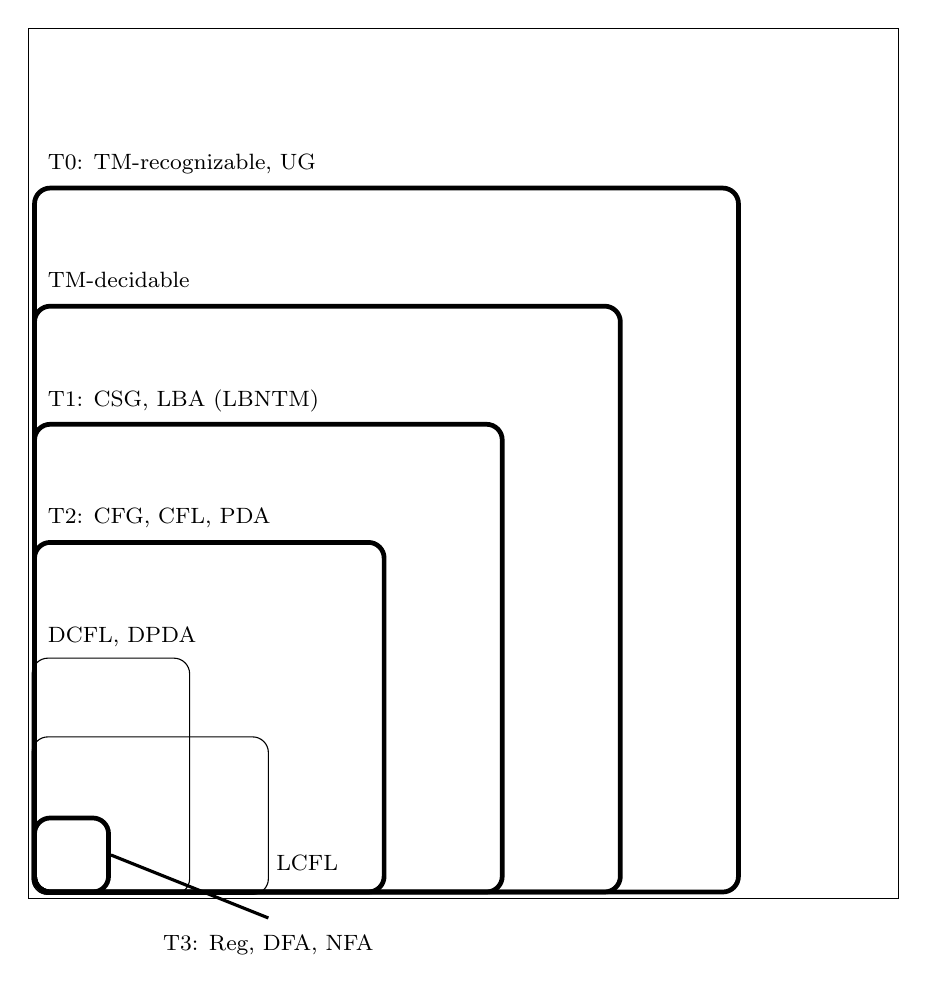
\begin{tikzpicture}

\draw (5.475, 5.475)
  node[draw, , , color=black,
       rounded corners=0cm, inner sep=0cm] {

\begin{minipage}[t][11.05cm]{11.05cm}
\mbox{}

\end{minipage}

};
\draw (0.5, 0.5)
  node[draw, line width=0.06cm, , color=black,
       rounded corners=0.2cm, inner sep=0cm] {

\begin{minipage}[t][0.94cm]{0.94cm}
\mbox{}

\end{minipage}

};
\draw (3.0, -0.65)
  node[draw=none, line width=0cm, , color=black,
       rounded corners=0cm, inner sep=0cm] {

\begin{minipage}[t][0.7cm]{2cm}
\mbox{}

\end{minipage}

};\draw (3.0, -0.65) node[color=black] {{\footnotesize T3: Reg, DFA, NFA}};\draw[line width=0.04cm,black] (1,0.5) to  (3.0,-0.3);

\draw (1.0, 1.5)
  node[draw, , , color=black,
       rounded corners=0.2cm, inner sep=0cm] {

\begin{minipage}[t][3.0cm]{2.0cm}
\mbox{}

\end{minipage}

};
\draw (2.6, 3.3)
  node[draw=none, line width=0cm, , color=black,
       rounded corners=0cm, inner sep=0cm] {

\begin{minipage}[t][0.1cm]{4.8cm}
\mbox{}

\end{minipage}

};
\draw (2.6, 3.3) node[color=black,
 inner sep=0cm] {
 
\begin{minipage}[t][0.1cm]{4.8cm}
{\footnotesize DCFL, DPDA}
\end{minipage}

};
\draw (1.5, 1.0)
  node[draw, , , color=black,
       rounded corners=0.2cm, inner sep=0cm] {

\begin{minipage}[t][2.0cm]{3.0cm}
\mbox{}

\end{minipage}

};
\draw (4.1, 0.4)
  node[draw=none, line width=0cm, , color=black,
       rounded corners=0cm, inner sep=0cm] {

\begin{minipage}[t][0.1cm]{2.0cm}
\mbox{}

\end{minipage}

};
\draw (4.1, 0.4) node[color=black,
 inner sep=0cm] {
 
\begin{minipage}[t][0.1cm]{2.0cm}
{\footnotesize LCFL}
\end{minipage}

};
\draw (2.25, 2.25)
  node[draw, line width=0.06cm, , color=black,
       rounded corners=0.2cm, inner sep=0cm] {

\begin{minipage}[t][4.44cm]{4.44cm}
\mbox{}

\end{minipage}

};
\draw (2.85, 4.8)
  node[draw=none, line width=0cm, , color=black,
       rounded corners=0cm, inner sep=0cm] {

\begin{minipage}[t][0.1cm]{5.3cm}
\mbox{}

\end{minipage}

};
\draw (2.85, 4.8) node[color=black,
 inner sep=0cm] {
 
\begin{minipage}[t][0.1cm]{5.3cm}
{\footnotesize T2: CFG, CFL, PDA}
\end{minipage}

};
\draw (3.0, 3.0)
  node[draw, line width=0.06cm, , color=black,
       rounded corners=0.2cm, inner sep=0cm] {

\begin{minipage}[t][5.94cm]{5.94cm}
\mbox{}

\end{minipage}

};
\draw (2.85, 6.3)
  node[draw=none, line width=0cm, , color=black,
       rounded corners=0cm, inner sep=0cm] {

\begin{minipage}[t][0.1cm]{5.3cm}
\mbox{}

\end{minipage}

};
\draw (2.85, 6.3) node[color=black,
 inner sep=0cm] {
 
\begin{minipage}[t][0.1cm]{5.3cm}
{\footnotesize T1: CSG, LBA (LBNTM)}
\end{minipage}

};
\draw (3.75, 3.75)
  node[draw, line width=0.06cm, , color=black,
       rounded corners=0.2cm, inner sep=0cm] {

\begin{minipage}[t][7.44cm]{7.44cm}
\mbox{}

\end{minipage}

};
\draw (2.85, 7.8)
  node[draw=none, line width=0cm, , color=black,
       rounded corners=0cm, inner sep=0cm] {

\begin{minipage}[t][0.1cm]{5.3cm}
\mbox{}

\end{minipage}

};
\draw (2.85, 7.8) node[color=black,
 inner sep=0cm] {
 
\begin{minipage}[t][0.1cm]{5.3cm}
{\footnotesize TM-decidable}
\end{minipage}

};
\draw (4.5, 4.5)
  node[draw, line width=0.06cm, , color=black,
       rounded corners=0.2cm, inner sep=0cm] {

\begin{minipage}[t][8.94cm]{8.94cm}
\mbox{}

\end{minipage}

};
\draw (2.85, 9.3)
  node[draw=none, line width=0cm, , color=black,
       rounded corners=0cm, inner sep=0cm] {

\begin{minipage}[t][0.1cm]{5.3cm}
\mbox{}

\end{minipage}

};
\draw (2.85, 9.3) node[color=black,
 inner sep=0cm] {
 
\begin{minipage}[t][0.1cm]{5.3cm}
{\footnotesize T0: TM-recognizable, UG}
\end{minipage}

};
\end{tikzpicture}

\end{center}



If you search for \texttt{6} in the BST above using BST search you will
visit the same values if you perform binary search on the sorted array for
\texttt{6}.


\newpage
\begin{ex}
Perform BST search on the above tree to look for \texttt{6}
and note down
the values you visit.
Now do binary search on the sorted array to look for \texttt{6}.
Maker sure you visit the same values in both cases.
Do the same for \texttt{0}.
\qed
\end{ex}


\newpage
Same runtime performance!

Remember ... the memory usage of array is not good if the array size
is big because you need a huge contiguous chunk of memory to satisfy
the memory allocation.
That's why we used nodes, forming a linked list.
\textit{But} ... the problem with the linked list is that
although memory usage is great, binary search is not possible.
Search for a value in a linked list is $O(n)$ in the worst case.
It's true that in the case of a BST search, \text{if}
the tree is roughly balanced (which is the average case),
the BST search has an average runtime of
\[
O(\log n)
\]

But that's not the end of the story:
Insert and delete for an array (sorted or not)
is in the average/worst case
\[
O(n)
\]
But if a BST tree is balanced (which is the average),
the insert and delete are both
\[
O(\log n)
\]
It does have a worst case of $O(n)$.

Everything is perfect and in the average case,
insert, delete, and search are all
\[
O(\log n)
\]
Meaning to say that average over all BST of size $n$,
the above runtimes hold.
\texttt{But} ... if you're always working with
\texttt{one} fixed BST that is heavily unbalanced,
then you're out of luck.
The question is then ... can we force a tree to be balanced?
